\documentclass[11pt,a4paper,bibtotoc,idxtotoc,headsepline,footsepline,footexclude,BCOR12mm,DIV13,hidelinks]{scrbook}


% Second template
% Set here the title, authors and other stuff to be used for the cover
% This file is used by MAIN.TEX

% set title, authors and stuff for the cover
\def\doctype{Master Thesis in Informatics}
\def\title{Adding C++ Support to MBEDDR}
\def\titleGer{C++ Unterst\"utzung f\"ur MBEDDR}
\def\author{Zaur Molotnikov}
\def\date{September 15, 2013}
\def\dateGer{15. September 2013}
\def\advisor{Dr. Daniel Ratiu}
\def\supervisor{Dr. Bernhard Sch\"atz}

% text to appear in the footer
\def\footertext{}
% include settings
% Included by MAIN.TEX
% Defines the settings for the CAMP report document

\renewcommand{\sectfont}{\normalfont \bfseries}        % Schriftart der Kopfzeile

% manipulate footer
\usepackage{scrpage2}
\pagestyle{scrheadings}
\ifoot[\footertext]{\footertext} % \footertext set in INFO.TEX
%\setkomafont{pagehead}{\normalfont\rmfamily}
\setkomafont{pagenumber}{\normalfont\rmfamily}

%% allow sophisticated control structures
\usepackage{ifthen}

% use Palatino as default font
\usepackage{palatino}

% enable special PostScript fonts
\usepackage{pifont}

% make thumbnails
\usepackage{thumbpdf}

%to use the subfigures
\usepackage{subfigure}


\usepackage{colortbl}


%% show program code\ldots
%\usepackage{verbatim}
%\usepackage{program}

%% enable TUM symbols on title page
\usepackage{styles/tumlogo}


\usepackage{multirow}

%% use colors
\usepackage{color}

%% make fancy math
\usepackage{amsmath}
\usepackage{amsfonts}
\usepackage{amssymb}
\usepackage{textcomp}
\usepackage{yhmath} % f�r die adots 
%% mark text as preliminary
%\usepackage[draft,german,scrtime]{prelim2e}

%% create an index
\usepackage{makeidx}

% for the program environment
\usepackage{float}

%% load german babel package for german abstract
%\usepackage[german,american]{babel}
\usepackage[german,english]{babel}
\selectlanguage{english}

% use german characters as well
\usepackage[latin1]{inputenc}       % allow Latin1 characters

% use initals dropped caps - doesn't work with PDF
%\usepackage{dropping}


\usepackage{styles/shortoverview}
%----------------------------------------------------
%      Graphics and Hyperlinks
%----------------------------------------------------

%% check for pdfTeX
\ifx\pdftexversion\undefined
 %% use PostScript graphics
 \usepackage[dvips]{graphicx}
 \DeclareGraphicsExtensions{.eps,.epsi}
 \graphicspath{{figures/}{figures/review}} 
 %% allow rotations
 \usepackage{rotating}
 %% mark pages as draft copies
 %\usepackage[english,all,light]{draftcopy}
 %% use hypertex version of hyperref
 \usepackage[hypertex,hyperindex=false,colorlinks=false]{hyperref}
\else %% reduce output size \pdfcompresslevel=9
 %% declare pdfinfo
 %\pdfinfo { 
 %  /Title (my title) 
 %  /Creator (pdfLaTeX) 
 %  /Author (my name) 
 %  /Subject (my subject	) 
 %  /Keywords (my keywords)
 %}
 %% use pdf or jpg graphics
 \usepackage[pdftex]{graphicx}
 \DeclareGraphicsExtensions{.jpg,.JPG,.png,.pdf,.eps}
 \graphicspath{{figures/}} 
 
 %% Load float package, for enabling floating extensions
 \usepackage{float}
 
 %% allow rotations
 \usepackage{rotating}
 %% use pdftex version of hyperref
 \usepackage[pdftex,colorlinks=false,linkcolor=black,citecolor=black,%
 anchorcolor=black,urlcolor=black,bookmarks=true,%
 bookmarksopen=true,bookmarksopenlevel=0,plainpages=false%
 bookmarksnumbered=true,hyperindex=false,pdfstartview=%
 ]{hyperref}
%
%\usepackage[pdftex,colorlinks=false,linkcolor=red,citecolor=red,%
% anchorcolor=red,urlcolor=red,bookmarks=true,%
% bookmarksopen=true,bookmarksopenlevel=0,plainpages=false%
% bookmarksnumbered=true,hyperindex=false,pdfstartview=%
% ]{hyperref}
\fi


%For C++ stuff
\usepackage{listings}

%% Fancy chapters
%\usepackage[Lenny]{fncychap}
%\usepackage[Glenn]{fncychap}
%\usepackage[Bjarne]{fncychap}

%\usepackage[avantgarde]{quotchap}

% set the bibliography style
%\bibliographystyle{styles/bauermaNum}
%\bibliographystyle{alpha}
\bibliographystyle{unsrt}

% To control where figure go
\usepackage[section]{placeins}

% For the gloassary
\usepackage[toc]{glossaries}


% include commands
% Commands to be used within the TUM report document
% Included by MAIN.TEX
% Please include your own cool commands here. 
% Be only sure to comment it sufficiently so others can use it.

%-------------------------------------------------------------
%                      Own Commands
%-------------------------------------------------------------


%-------------------------------------------------------------
% math stuff -------------------------------------------------

% nice R, N, C
\newcommand{\nat}{\mathbb{N}}
\newcommand{\real}{\mathbb{R}}
\newcommand{\compl}{\mathbb{C}}



% norm
\newcommand{\norm}[1]{\left\| #1 \right\|}

% un demi
\newcommand{\half}{\frac{1}{2}}

% parantheses
\newcommand{\parenth}[1]{ \left( #1 \right) }
\newcommand{\bracket}[1]{ \left[ #1 \right] }
\newcommand{\accolade}[1]{ \left\{ #1 \right\} }
%\newcommand{\angle}[1]{ \left\langle  #1 \right\rangle }

% partial derivative: %#1 function, #2 which variable
% simple / single line version
\newcommand{\pardevS}[2]{ \delta_{#1} f(#2) }
% fraction version
\newcommand{\pardevF}[2]{ \frac{\partial #1}{\partial #2} }

% render vectors: 3 and 4 dimensional
\newcommand{\veciii}[3]{\left[ \begin{array}[h]{c} #1 \\ #2 \\ #3	\end{array} \right]}
\newcommand{\veciv}[4]{\left[ \begin{array}[h]{c} #1 \\ #2 \\ #3 \\ #4	\end{array} \right]}

% render matrices: 3  dimensional (arguments in row first order)
\newcommand{\matiii}[9]{\left[ \begin{array}[h]{ccc} #1 & #2 & #3 \\ #4 & #5 & #6 \\ #7 & #8 & #9	\end{array} \right]}
%DOESN'T WORK,DON'T KNOW WHY \newcommand{\mativ}[16]{\left[ \begin{array}[h]{cccc} #1 & #2 & #3 & #4 \\ #5 & #6 & #7 & #8 \\ #9 & #10 & #11 & #12 \\ #13 & #14 & #15 & #16 \end{array} \right]}


%-------------------------------------------------------------
%-------------------------------------------------------------


%-------------------------------------------------------------
% some abreviations ------------------------------------------
\newcommand{\Reg}{$^{\textregistered}$}
\newcommand{\reg}{$^{\textregistered}$ }
\newcommand{\Tm}{\texttrademark}
\newcommand{\tm}{\texttrademark~}
\newcommand {\bsl} {$\backslash$}

%-------------------------------------------------------------
%-------------------------------------------------------------


%-------------------------------------------------------------
% formating --------------------------------------------------

% Theorem & Co environments and counters
\newtheorem{theorem}{Theorem}[chapter]
\newtheorem{lemma}[theorem]{Lemma}
\newtheorem{corollary}[theorem]{Corollary}
\newtheorem{remark}[theorem]{Remark}
\newtheorem{definition}[theorem]{Definition}
\newtheorem{equat}[theorem]{Equation}
\newtheorem{example}[theorem]{Example}
\newtheorem{algorithm}[theorem]{Algorithm}

% inserting figures
\newcommand{\insertfigure}[4]{ % Filename, Caption, Label, Width percent of textwidth
	\begin{figure}[htbp]
		\begin{center}
			\includegraphics[width=#4\textwidth]{#1}
		\end{center}
		\vspace{-0.4cm}
		\caption{#2}
		\label{#3}
	\end{figure}
}




% referecing figures

\newcommand{\refFigure}[1]{ %label
	figure \ref{#1}
}
\newcommand{\refChapter}[1]{ %label
	chapter \ref{#1}
}

\newcommand{\refSection}[1]{ %label
	section \ref{#1}
}

\newcommand{\refParagraph}[1]{ %label
	paragraph \ref{#1}
}

\newcommand{\refEquation}[1]{ %label
	equation \ref{#1}
}

\newcommand{\refTable}[1]{ %label
	table \ref{#1}
}




\newcommand{\rigidTransform}[2]
{
	${}^{#2}\!\mathbf{H}_{#1}$
}

%code, in typewriter
\newcommand{\code}[1]
 {\texttt{#1}}

% comment that appears on the border - very practical !!!
\newcommand{\comment}[1]{\marginpar{\raggedright \noindent \footnotesize {\sl #1} }}

% page clearing
\newcommand{\clearemptydoublepage}{%
  \ifthenelse{\boolean{@twoside}}{\newpage{\pagestyle{empty}\cleardoublepage}}%
  {\clearpage}}


%-------------------------------------------------------------
%-------------------------------------------------------------


\newcommand{\etAl}{\emph{et al.}\mbox{ }}

% Listings of C++ code
\newcommand{\cpp}[2]{\begin{center}\lstset{caption=#1, frame=tb, label={lst:#2}}\lstinputlisting[language=C++]{listings/#2.cpp}\end{center}\FloatBarrier}
\newcommand{\rl}[1]{Listing \ref{lst:#1}}

% Inclusion of mps screenschots
%graphics
\newcommand{\gr}[3]{\begin{figure}[!ht, #1]\centering\includegraphics[scale=#3]{#1}\caption{#2}\label{fig:#1}\end{figure}}
%MPS Screenshot
\newcommand{\ms}[2]{\gr{#1}{#2}{0.27}\FloatBarrier}
\newcommand{\msnozoom}[2]{\gr{#1}{#2}{0.77}\FloatBarrier}
\newcommand{\fig}[1]{Figure~\ref{fig:#1}}

%C/C++ code inline
\newcommand{\cc}[1]{\texttt{#1}}

%Reference a part
\newcommand{\rpart}[1]{Part\ \ref{part:#1}}

%Reference a chapter
\newcommand{\lchap}[1]{\label{chapter:#1}}
\newcommand{\declchap}[2]{\chapter{#1}\lchap{#2}}
\newcommand{\rchap}[1]{Chapter\ \ref{chapter:#1}}



%Reference a section
\newcommand{\lsec}[1]{\label{section:#1}}
\newcommand{\rsec}[1]{Section \ref{section:#1}}


%Reference a special goal
\newcommand{\rsgoal}[1]{Special Goal #1 (see \ref{g#1})}

%Glossary things
\newcommand{\rg}[1]{\emph{\gls{#1}}}
\newcommand{\Rg}[1]{\emph{\Gls{#1}}}
% include custom abbreviations
%My own command to use in the text as abbreviations

\newcommand{\mbdr}{\rg{mbeddr}}
\newcommand{\mb}{\mbdr}
\newcommand{\mbeddr}{\mbdr}

\newcommand{\mbdp}{\rg{mbeddrproject}}
\newcommand{\mbdrp}{\mbdp}
\newcommand{\mbp}{\mbdp}

\newcommand{\MT}{Master Thesis}

\newcommand{\cpppl}{C++ programming language}

\newcommand{\jbmps}{\Rg{mps}}

% include the glossary
\newglossaryentry{abstract}
{
  name=abstract,
  description={ a class in C++, having at least one method declared pure virtual in ancestors, but never implemented in the ancestors or the
  class itself, instances of such class can not be created}
}

\newglossaryentry{acsa}
{
  name=abstract class syntax absence,
  description={ a phenomenon in C++, consisting in absence of any syntax to explicitly declare a class abstract}
}

\newglossaryentry{action}
{
  name=action,
  description={ is a JetBrains MPS term, which corresponds to a automations, specific to actions, occurring while editing}
}




\newglossaryentry{analysisondemand}
{
  name=analysis-on-demand,
  plural=analyses-on-demand,
  description={ is an analysis, which the user must invoke explicitly in the \rg{ide}, it is usually computationally expensive, c.f. 
  \rg{selfrunninganalysis} }
}


\newacronym{api}{API}{Application Programming Interface}

\newacronym{ast}{AST}{Abstract Syntax Tree}

\newglossaryentry{baseconcept}
{
  name=base concept,
  description={ is a JetBrains MPS concept, which serves as an inheritance base or parent concept for a given concept, e.g. 
  Statement concept for IfStatement concept}
}


\newglossaryentry{concept}
{
  name=concept,
  description={ is a class-like type, describing a node type in the \rg{ast} when talking about projectional editing}
}


\newacronym{dsl}{DSL}{Domain Specific Language}


\newglossaryentry{emcpp}
{
  name=Embedded C++,
  description={ is a language subset of the C++ programming language, intended to
  support embedded software development}
}

\newglossaryentry{exemcpp}
{
  name=Extended Embedded C++,
  description={ is a improvement of Embedded C++, bringing back the omitted language features, and a memory-aware \rg{stl} version}
}

\newglossaryentry{informativeanalysis}
{
  name=informative analysis,
  plural=informative analyses,
  description={ is performed to inform the user about some code properties, to enhance understanding of the code and its properties}
}

\newacronym{ide}{IDE}{Integrated Development Environment}

\newglossaryentry{intention}
{
  name=intention,
  description={ is a special procedure in \jbmps\ which can be used for automatic manipulations on the \rg{ast} with a 
  node of a given \rg{concept}}
}

\newglossaryentry{interfaceconcept}
{
  name=interface concept,
  description={ is a JetBrains MPS concept, which serves for inheriting a concept behavior interface, can not serve as a base concept}
}


\newglossaryentry{mbeddr}
{
  name=mbeddr,
  description={ same as mbeddr project}
}


\newglossaryentry{mbeddrproject}
{
  name=mbeddr project,
  description={ is a JetBrains MPS based language workbench, representing C language and domain specific
  extensions for the embedded software development}
}

\newglossaryentry{model}
{
  name=model,
  description={ correspond to one single JetBrains MPS file unit, in the mbeddr context it corresponds 
  to C or C++ project, like one library or one executable.}
}

\newglossaryentry{mps}
{
  name=JetBrains MPS,
  description={ is a language engineering environment 
  allowing to construct incrementally defined domain specific languages}
}

\newglossaryentry{ovsa}
{
  name=override syntax absence,
  description={ a phenomenon in C++, consisting in absence of any syntax to explicitly designate a method, being an override
  of another method}
}


\newglossaryentry{preventiveanalysis}
{
  name=preventive analysis,
  plural=preventive analyses,
  description={ is performed to inform the user about the potential mistakes in advance, in order to prevent them}
}

\newglossaryentry{projectionalapproach}
{
  name=projectional approach,
  description={ is an approach to create an editor for a language, when the editor is 
  aware of the \rg{ast} for the code, and shows the code to the user, projecting the 
  \rg{ast} itself, and allowing to edit the \rg{ast} directly}
}

\newglossaryentry{projectionalcpp}
{
  name=Projectional C++,
  description={ a C++ flavor introduced by this work, based on mbeddr C++ implementation in the JetBrains MPS environment}
}

\newglossaryentry{purevirtual}
{
  name=pure virtual,
  description={ are methods in a C++ class, for which intentionally no implementation is provided, they serve purely for overloading purposes, 
  describing a pure interface}
}


\newglossaryentry{selfrunninganalysis}
{
  name=self-running analysis,
  plural=self-running analyses,
  description={ is an analysis, which determines itself the point of time, when it is performed, or this moment is determined automatically
  by the \rg{ide},   there is no need to explicitly run such analysis}
}

\newacronym{stl}{STL}{Standard Template Library}

\newglossaryentry{textgen}
{
  name=TextGen,
  description={ is an special kind of generator in JetBrains MPS, dedicated to produce a textual representation of a node of a given concept}
}

\makeglossaries

\begin{document}

	\frontmatter
	
	
	% The front cover for the TUM report document.
% Included by MAIN.TEX


%--------------------------------------------------
% The Front Cover
%--------------------------------------------------

% The front cover for the TUM document.
% Included by MAIN.TEX


%--------------------------------------------------
% The Front Cover
%--------------------------------------------------

% correct BCOR - undo at the end !!!
\def\bcorcor{0.15cm}
\addtolength{\hoffset}{\bcorcor}

\thispagestyle{empty}

 \vspace{4cm}
\begin{center}
	       \oTUM{4cm}
	   
	   \vspace{5mm}     
	   \huge FAKULT{\"A}T F{\"U}R INFORMATIK\\ 
	   \vspace{0.5cm}
	 \large DER TECHNISCHEN UNIVERSIT{\"A}T M{\"U}NCHEN\\
    \vspace{1mm}
        
	\end{center}
		

\vspace{15mm}
\begin{center}

   {\Large \doctype}

  \vspace{20mm}
  
  {\huge\bf \title}\\%[3ex]
  
  
  \vspace{15mm}
  
  
  {\LARGE  \author}
  
  \vspace{10mm}
  
  \begin{figure}[h!]
  \centering
   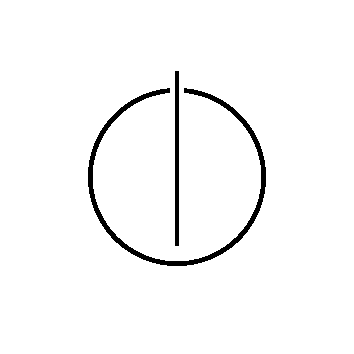
\includegraphics[width=4cm]{styles/informat.png}
  \end{figure}
  
  \end{center}
%	\clearemptydoublepage
%	
%	% The titlepage for the CAMP report document.
% Included by MAIN.TEX


%--------------------------------------------------
% The title page
%--------------------------------------------------

% correct BCOR - undo at the end !!!
\def\bcorcor{0.15cm}
\addtolength{\hoffset}{\bcorcor}

\thispagestyle{empty}

 \vspace{10mm}
\begin{center}
	       \oTUM{4cm}
	   
	   \vspace{5mm}     
	   \huge FAKULT{\"A}T F{\"U}R INFORMATIK\\ 
	   \vspace{0.5cm}
	 \large DER TECHNISCHEN UNIVERSIT{\"A}T M{\"U}NCHEN\\
        
	\end{center}
		

\vspace{10mm}
\begin{center}

   {\Large \doctype}

  \vspace{10mm}
  
  {\LARGE \title}\\
  
  
  \vspace{10mm}
  
  
  {\LARGE  \titleGer}\\
  
  
  \vspace{10mm}

    %\hfill
    \begin{tabular}{ll}
	   \Large Author:     & \Large \author \\[2mm]
	   \Large Supervisor:    & \Large \supervisor \\[2mm]				
	   \Large Advisor:	& \Large \advisor  \\[2mm]
	   \Large Date:       & \Large \date
	 \end{tabular}
	 
	 \vspace{5mm}
	 
	 \begin{figure}[h!]
  \centering
   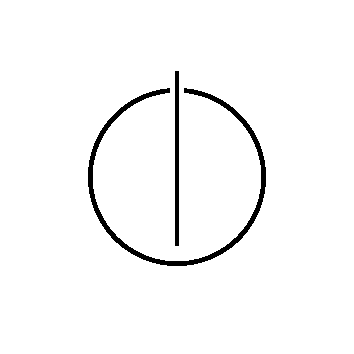
\includegraphics[width=4cm]{styles/informat.png}
  \end{figure}
   

\end{center}

% undo BCOR correction
\addtolength{\hoffset}{\bcorcor}
	
	
%	\input{components/cover_maschmeyer}
	\clearemptydoublepage
	
	% The titlepage for the CAMP report document.
% Included by MAIN.TEX


%--------------------------------------------------
% The title page
%--------------------------------------------------

% correct BCOR - undo at the end !!!
\def\bcorcor{0.15cm}
\addtolength{\hoffset}{\bcorcor}

\thispagestyle{empty}

 \vspace{10mm}
\begin{center}
	       \oTUM{4cm}
	   
	   \vspace{5mm}     
	   \huge FAKULT{\"A}T F{\"U}R INFORMATIK\\ 
	   \vspace{0.5cm}
	 \large DER TECHNISCHEN UNIVERSIT{\"A}T M{\"U}NCHEN\\
        
	\end{center}
		

\vspace{10mm}
\begin{center}

   {\Large \doctype}

  \vspace{10mm}
  
  {\LARGE \title}\\
  
  
  \vspace{10mm}
  
  
  {\LARGE  \titleGer}\\
  
  
  \vspace{10mm}

    %\hfill
    \begin{tabular}{ll}
	   \Large Author:     & \Large \author \\[2mm]
	   \Large Supervisor:    & \Large \supervisor \\[2mm]				
	   \Large Advisor:	& \Large \advisor  \\[2mm]
	   \Large Date:       & \Large \date
	 \end{tabular}
	 
	 \vspace{5mm}
	 
	 \begin{figure}[h!]
  \centering
   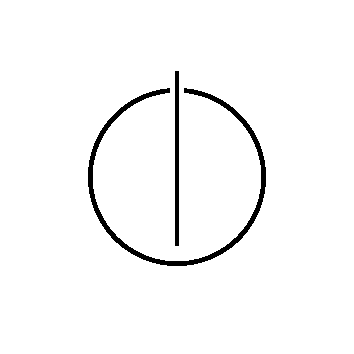
\includegraphics[width=4cm]{styles/informat.png}
  \end{figure}
   

\end{center}

% undo BCOR correction
\addtolength{\hoffset}{\bcorcor}
		
	\clearemptydoublepage


\thispagestyle{empty}
\selectlanguage{german}
	\vspace*{0.8\textheight}
	\noindent
	Ich versichere, dass ich diese Masterarbeit selbst{\"a}ndig verfasst und nur 
	die angegebenen \\Quellen und Hilfsmittel verwendet habe.
	
	\vspace{15mm}
	\noindent
	M{\"u}nchen, den \dateGer \hspace{5cm} \author
\selectlanguage{english}
\newpage
	
	\clearemptydoublepage
\phantomsection
\addcontentsline{toc}{chapter}{Acknowledgements}	


%\chapter*{Acknowledgements}

\vspace*{2cm}

\begin{center}
{\Large \bf Acknowledgments}
\end{center}

\vspace{1cm}




If someone contributed to the thesis... might be good to thank them here.
	
	% Abstract for the TUM report document
% Included by MAIN.TEX


\clearemptydoublepage
\phantomsection
\addcontentsline{toc}{chapter}{Abstract}	





\vspace*{2cm}
\begin{center}
{\Large \bf Abstract}
\end{center}
\vspace{1cm}

In this work we describe the process of adding the \cpppl\ support to \mbdp, an implementation of the
C programming language with extensions in a projectional language engineering environment, \jbmps. 
While implementing the \cpppl\ several well-known pitfalls of the language are taken into account
in an attempt to build a better C++ language flavor. Various analyses are implemented to improve
the programming experience for the end user. Lessons learned from this experience are described finally.
They include generalized principles, which could be used to improve a language while recreating it in a 
projectional language engineering environment; support of language modularity and extensibility  by \jbmps;
problems of building analyses and their complexity together with potential ways to resolve them in the future.

	\tableofcontents
  
  %% \clearemptydoublepage
% 
% \phantomsection
% \addcontentsline{toc}{chapter}{Outline of the Thesis}
% 
% \begin{center}
% 	\huge{Outline of the Thesis}
% \end{center}
% 
% 
% 
% 
% %--------------------------------------------------------------------
% \section*{Part I: Introduction and Theory}
% 
% \noindent {\scshape Chapter 1: Introduction}  \vspace{1mm}
% 
% \noindent  This chapter presents an overview of the thesis and it purpose. Furthermore, it will discuss the sense of life in a very general approach.  \\
% 
% \noindent {\scshape Chapter 2: Theory}  \vspace{1mm}
% 
% \noindent  No thesis without theory.   \\
% 
% %--------------------------------------------------------------------
% \section*{Part II: The Real Work}
% 
% \noindent {\scshape Chapter 3: Overview}  \vspace{1mm}
% 
% \noindent  This chapter presents the requirements for the process.

	\mainmatter
	
	
		% ---------------------------------------------------------------------------
		%
		% Introduction to the problem
		%
		% ---------------------------------------------------------------------------
		%\part[Introduction and Theory]{Introduction and Theory}
		%\label{part:intro}
		\declchap{Introduction}{intro}

\section{Context}

In embedded programming the C++ programming language is widely spread, \cite{embedlangs}. Being a general purpose 
programming language, C++ does not provide, however, any special support for embedded systems programmers. 

By changing  the language itself, together with a tool set for it, it is possible to get a better environment 
for a dedicated domain, for example, specifically for embedded programming. There are two known approaches to change
the language itself.

The first possible approach is dropping some language features, to get the language, which is simpler. 
As an example, a subset of C++, called \Rg{emcpp} can be brought, \cite{emcpp}. The approach taken in \Rg{emcpp} is 
omitting very many core features of C++ like virtual base classes, exceptions, namespaces and templates. 
It allows for a higher degree of optimizations by compiler possible. 

\Rg{emcpp} was intended to ensure higher software quality through better understanding of the limited 
C++ by programmers, higher quality of compilers, through simplicity, better suitability for the embedded domain, through
memory consumption considerations \cite{stripepp}. 

The C++ community has criticized the approach taken in \Rg{emcpp}, specifically for the inability of the 
limited language to take advantage of the C++ \rg{stl}, which requires the C++ language features, absent in 
\Rg{emcpp}, \cite{stremcpp}. As a response for it IAR Systew have developed \rg{exemcpp}, which includes many of the language features,
omitted by \Rg{emcpp}, and a memory-aware version of \rg{stl}, \cite{extendedembeddedcpp}.

The second approach to modify a language in order to get it more suitable for embedded development consists of extending 
the language with constructions, specific to the domain. The authors of the \mbdp\ has taken such approach, to improve on
the C programming language, \cite{2012_voelter_mbeddr_extensible_c_based_language_and_ide_for_embedded}. 

Specific extensions may represent some often met idioms in the domain, for example, 
a state table or  a state machine diagram in a specification may describe behavior of a device under the 
programmer control. A language developer can incorporate such notions as a sate machine into a language, \fig{dectab}\footnote{Illustration is taken from \cite{2012_ratiu_modular_dsls_and_analyses} }, 
providing a higher abstraction level, when compared to the existing language constructs. 

\gr{dectab}{Example of a Decision Table, Added to C Language}{1.0}

Moreover, higher level extensions induce some higher level semantics. An \rg{ide} under construction could check 
this higher level semantics for correctness on the programming stage. For example, an \rg{ide} can check a given decision table 
for completeness of choices and their consistency, \cite{2012_ratiu_modular_dsls_and_analyses}. Such checks can improve 
quality of the software under development. 

Extensions to C language developed in \rg{mbeddr} include state machines and decision tables, together with analyses
for them.

For example, the \fig{dectab} demonstrates a decision table. The decision table takes \cc{mode} and \cc{speed} as input parameters
and returns a new \cc{mode} value as determined by the input parameters. A careful reader can see, that the exact value \cc{30} of \cc{speed}
is not taken into account, and the default value \cc{FAIL} is going to be returned. A programmer could invoke analysis\footnote{Described in detail 
in  \cite{2012_ratiu_modular_dsls_and_analyses}}, to find out that the table is not covering itself the whole choice space.

The \mbdr\ development team have used a special language engineering environment, \Rg{mps}, to support modular and incremental 
language development.  A programmer using \jbmps\ splits a language under development into special class-like items, 
called \rgp{concept}. Concepts represent the \rg{ast} node types. 

As an example of a \rg{concept} an expression can be taken. It is possible to describe in \Rg{mps} different 
expression kinds, similar to object oriented class hierarchy, allowing the objects to reference each other, 
and enabling polymorphism, in a way when any descendant can be used instead of its ancestor, e.g. 
binary minus expression can be used wherever an expression (any expression) is required. 
After various expression types were described to the language engineering environment as \rgp{concept}, 
the environment provides a chance to instantiate concrete expressions and edit them, acting as an editor for 
the language created.

Over the inheritance mechanisms, it is possible to extend languages, providing new concepts as descendants of 
the existing ones. For example, expression concept can be extended to support new sort of expressions, like decision tables.
Thus language modularity is achieved and incremental development is made to be possible.

Modularity is achieved as well, when one language is enabled to interact with another one. For example, expressions,
described independently as a language, can be reused in any language, which has a need in expressions, like language with
statements of a programming language, because statements include expressions naturally.

Having in mind the opportunities, the language modularity in \jbmps\ brings, it makes sense to recreate a general 
purpose programming language in \jbmps. Building the general purpose programming language brings a basis to develop 
domain specific extensions to the well-known general purpose language. The editor for the general purpose language comes 
almost ``for free'', as a side product. 

Later, from the code in the implemented general purpose language a text code can be generated for further processing, 
compiling, deployment. The language extensions, of-course, are not known to the existing tools which process the language.
But they usually can be reduced to the base general purpose programming language statements, presenting a regular 
syntax to the further tool chains as an outcome. Thus the general purpose programming language is getting enhanced,
remaining compatible with all the existing tools to process it further.

Additionally to the language modification itself, an \rg{ide} can be improved to support the domain specific 
development. 

Various analyses\footnote{analyses not only for extensions, but for the base language itself} 
can be built in into the code editor in order to detect inconsistencies, or, simply, ``dangerous'' constructs, 
and inform the programmer. Certain code formatting, or standard requirements could be enforced as well. 
The \rg{ide} can be enhanced with various automations, like support for code generation and refactorings. 

As the new \rg{ide} works internally with \rg{ast} described through the node types, or \rgp{concept}, in order to perform code
analysis, generation, or transformation, there is no need to invoke parsers for the code, which is advantageous.

\section{Problem}
A mixture of the two approaches is used in this work in an attempt to achieve a modular C++ language, a suitable base for the 
further language engineering, including the specialization  of C++ for embedded development, and even more general, 
for later extension, to specialize the common base C++ language to any domain of choice. A special \rg{ide} is created 
together with a new C++ language flavor, which supports the C++ programmer.

During the creation of the \cpppl\ in the way described, the language modularity in general is analyzed, and caveats of it
are described together with the ways to avoid them.

The newly created \rg{ide} features analyses. The question of their computational complexity for such analyses 
is raised in general, together with the practical outcomes of it.

The new language together with the new \rg{ide} can later serve as a basis for extending the C++ programming 
language with domain specific constructs for embedded programming. Creation of these extensions lies out of scope
for this Master Thesis, and is left for further research.

\section{Approach}
The approach taken in this work goes further into exploring the language modularity on the basis of \jbmps. While building 
the \cpppl\ itself  with the goal of embedded domain specific extensions in mind, the C++ itself is being built itself as 
an extension to the C programming language, provided by the \rg{mbeddr}. The C++ implemented in \jbmps\ and discussed in this 
work I call the \pcpp.

Although C++ is a separate from C language, the high degree of similarity allows to make use of the C programming language,
implemented by the \rg{mbeddr} as a foundation. Not only reuse of the basic C is achieved, but also the embedded extensions from
the \rg{mbeddr} are immediately supported by the newly built C++.

The ultimate goal during the reuse of \mbdr\ as a base for C++ is keeping \rg{mbeddr}
not modified towards the \cpppl\ only, but instead, making, when needed, \mbeddr\  more extensible in general, 
so that both resulting C++ and the base for it, \mbdr,  can develop further being disjoint to a high degree.
This independence of \mbdr\ on C++ extension ensures, that the \mbdp\ can develop further without looking back 
on C++, making the C++ support an independent task.

\section{Contribution}

In this work we describe a \cpppl\ implementation\footnote{This implementation does not represent complete C++, and
limitations are discussed along this work} on top of \mbdp.

The task of a one-side-aware only extension is a challenge for the whole language modularity concept, 
provided by \jbmps. This work explores further the support, provided by \jbmps\ for the modular 
language construction, c.f. \cite{2012_ratiu_modular_dsls_and_analyses}, and reviews it from the architectural point of view,
summarizing in the end the support for it, provided by \jbmps.

This work contributes the \cpppl\ with a number of automations and analyses for it. The automations include code 
generation and structuring. They are designed to compensate on some caveats of C++, or lack of support for 
several aspects in the language itself, like coding style. The analyses are intended to increase the understanding of the constructed
code by a novice to C++ programmer, or to provide a quick information to an experienced C++ professional. 
Both analyses and automations are provided to achieve an improvement in quality, security and understanding of 
the pure C++ code. The automations and analyses are mostly implemented as a programming on the \rg{ast} 
in a Java-like programming language.

As analyses and automations grow in complexity and quantity, the question of their computational complexity arises.
In the \jbmps\ \rg{api} it is not explicitly defined, when the analyses provided for the language take place, 
how much of the computational resource they can take advantage of, and how the end user should be informed on the results and progress. 
These aspects may affect the overall \rg{ide} behavior, including performance, as the analyses complexity may be high and the results of them could 
be of a high value. 
The question of analyses run-time, complexity and results presentation is raised and discussed in 
this work in general and in particular, suggesting improvements to \jbmps \rg{api}.

Finally, it is fair to say, that the \mbdr\ team\footnote{especially Markus Voelter} have already grounded some practical foundations for the \pcpp, 
before the start of this work. Some of them, were kept (reference type, templates partially) and just described and analyzed 
here, some of them were considerably reworked (classes, inheritance, encapsulation and polymorphism). 

Couching from the \mbdr\ team made me changing some of the implementation aspects to be different from what I planned originally (namespaces,
operator overloading partially). And, of-course, I built some parts new, from scratch, without any influence (at least at the moment of being) \mbdr\ team 
at all (all analyses, construction and copying, some more). 

The evaluation of the experience, gained by me during the practical implementation part, results into the extensibility analysis, 
research on complexity of checks and the run-time for them together with suggested \jbmps\ improvements, and general guidelines 
for building projectional language implementation represent my own theoretical focus and commitment.

\section{Structure of the \MT}


		
		
		% ---------------------------------------------------------------------------
		%
		% Theoretical foundations
		%
		% ---------------------------------------------------------------------------
		%\part[C++ and Projectional Editing]{C++ and Projectional Editing}
		%\label{part:implementation}
		\declchap{Foundations}{found}

Before describing the technologies on which the current work is based, as well as the work itself,
it makes sense to describe more general foundations and principles, around which the technology is built.

In the \rsec{dslsandides} we describe two approaches to create an \Rg{ide} for a certain language, and mainly the 
projectional approach, which originates from the area of building new \Rgp{dsl}.

In the \rsec{modularlang} we describe the modular approach towards language engineering and extending, intensively
used with the projectional approach to construct languages.

% TODO If more sections appear in this chapter - mention them here

\declsec{Building DSLs and IDEs}{dslsandides}

This section compares the traditional approach to build textual editors for the program code with
the projectional approach, bringing up  motivation for the least.

\subsection{Traditional Approach}
Traditionally programming languages are used in a textual form in text files, forming programs.
However the textual nature is not typical for the structure of programs themselves, being rather a low-level code representation, especially when talking abut syntax, which is only necessary for 
parsers to produce correct results, and not for the program intended semantics.

% About syntax trash here

Parsers are used to construct so-called \rg{ast}s from the textual 
program representation. \rg{ast}s are structures in memory, usually graph-alike, 
reminding a control flow graph, where nodes are different statements and edges are 
the ways control passes from one statement to the next one.

For the developer, using an editor, the degree to which the editor can support the development
process is important. For this, the editor has to recognize the programming language constructions and provide possible assistance. Among such assistance can be code formatting, syntax validation,
source code transformations (including refactoring support), code analyses and verification, 
source code generation and others. Many of these operation rely indeed on the higher than text level notions related to program such as a method, a variable, a statement. 
A good editor has to be aware of these higher level program structures, to provide meaningful automations for the operations mentioned above.

Nowadays, most of the editors work with text, and, to provide assistance to a programmer, integrate
with a parser/compiler front-end for the programming language. Such way to extract the program
structure during editing is not perfect for several reasons:

\begin{enumerate}
 \item The program being edited as text is not syntactically correct at every moment, 
being incomplete, for example. Under such circumstances the parsing front-end can not be
successfully invoked and returns error messages which are either not related to the program, when
the code is completed, or false-positive warning and errors. 
  
 \item After a minor editing of the code, usually the whole text file has to be processed again. Such compiler calls are usually 
computationally expensive, they slow down, sometimes significantly, the performance of the developer machine. Various techniques exist to speed it up, including partial 
and pre- compilation, but the problem is still relevant to a large extent. 

\item The textual nature of the code complicates certain operations additionally. As an example, we can take a refactoring
to rename a method. Every usage of the method, being renamed, has to be found and changed. To implement it correctly an editor must take into account various possible name collisions, as well 
as presume a compilable state of the program prior to the start of the refactoring.

\end{enumerate}

Not to mention the parsing problem itself. Parsing a program in a complex language like C++ is a difficult problem, it involves 
the need to resolve correctly scoping and typing, templates and related issues, work with pre-processor directives incorporated
in the code. In this regard different compilers treat C++ in a different way, creating dialects, which may represent obstacles for
the code to be purely cross-platform.

\cpp{Closing several blocks}{blocks}

The textual representation of program code, involves the need in formatting and preserving syntax. These both tasks, indeed,  have nothing to do with the functionality program, and additionally 
load the developer, reducing productivity. As an example, here we can mention the need to close
several blocks ending at the same point correctly, indenting the closing brace symmetrically 
to opening one. The \rl{blocks} demonstrates it in the last few lines.

\subsection{Projectional Approach}

Another approach a creator can take when building an \rg{ide}  is called \rg{projectionalapproach}. 
Projectional editors do not work with a low-level textual representation of a program, but rather with a higher level concept, \rg{ast}s.
This approach is especially useful and used when constructing new \rg{dsl}s.

Working with \rg{ast}s directly has several advantages over the conventional textual code editing:

\begin{enumerate}
 \item All syntax errors are no longer possible, as there is no syntax. 
 \item There is no need to format the code on the level of indentation and look, since it is only
needed for textual code.
  \item All features, which in textual approach require parsing, can be implemented without a parser involved, because \rg{ast} is always known to the editor.
\end{enumerate}

Additionally, as the compilers still expect a code in a textual form, code generation is used to
convert the \rg{ast} into the text code for the further use. The code generation step can be 
customized to provide support for a variety of compilers, when the compilers differ.

Projectional editors have to display the \rg{ast} to the developer, in order for him/her to work with it. Such visualization
of an \rg{ast} is called ``projection'', giving a name to the editor class.

The model of code is stored as an \rg{ast} in the projectional editor. As in the Model-View-Controller pattern the view for
the model can be implemented separately, \cite{GOF95}. Thus the code may be presented in a number of different ways to the user. For example, the \rg{ast} can be visualized as a graph, similar to control flow graph. This visualization, however, is not always advantageous being sometimes not compact and
complicated to overview.

\ms{constructor}{Example projection of an \rg{ast}, ``source code'' view}

One of the well-accepted way to visualize \rg{ast} is by visualizing its textual representation, as if
it would be written as a text code in the programming language, see \fig{constructor}. There can be in  
principle many such textual visualizations, supporting different ways the code looks. Normally in 
the traditional approach this has to be achieved by reformatting, and thus changing, the source code.
This is performed for the code to look similar across the developed software, and standards or coding 
guidelines are written to enforce the way to format the text code. Compare to the projectional approach,
where such formatting guidelines are not needed, when arguing about the low-level code formatting,
like indentation.

The textual projection of the \rg{ast} looks similar to the text code. However the projectional 
nature of it has certain outcomes, which may be unusual for a programmer, who is used to editing
the code as text.

The statements in the projectional editor are only selected as whole. There is now way to just select 
the ``while'' word for cut or copy, without selecting the condition and the block belonging to the statement. 
This behavior represents the position of the condition and \cc{while}-body in the \rg{ast} as children of the \cc{while} 
statement. The statement can be selected all together only, including all of its children. Alternatively, one could 
select just an expression in the condition part.

Every block delimiters are just a part of the block visualization. They are organized in a proper way
automatically, and there is no way to delete or confuse them, as well as to type them initially. Each
closing brace can marked with the parent statement name (through implementing such behavior in the
\rg{ast} visualization), enhancing navigation through the displayed code.

As one can see, the textual projection of the \rg{ast} looks almost the same, as a text code in a 
conventional textual editor. This can cause some confusion for the developer at first, 
as attempts to edit this textual visualization as a real text will sometimes fail. 

Eventually, however, advantages of such visualization overwhelm the disadvantages. 
Among the benefits of the textual projection over text code are quicker code construction 
after short learning, better way to select code fragments, since not individual 
characters or lines, but rather \rg{ast} nodes or groups of nodes are selected, 
plus, all the advantages, the projectional editing brings by itself, as discussed above.

we discuss additionally the projectional approach and some of its basic 
principles, which we consider to be of practical value in the \rsec{genprinciples}.

\declsec{Modular Language Engineering}{modularlang}

\subsection{Describing a Language in Projection}

When  building a projectional editor for a language, the language must be given as a certain description of the \Rg{ast}.
As \rg{ast} represent a graph, the nodes and edges types, as well as their possible relationships must be described\footnote{Compare this
with the textual approach, where a grammar for the language must be built, which is generally speaking complex, and some times even not a
possible task, which leads to the increasing parser complexity, known problem in particular in the C++ area}. 

The nodes of the \rg{ast} are described through giving their types. The node type in projectional editing is called a \rg{concept}. \Rgp{concept} are very
similar to classes in object oriented programming languages. They feature inheritance, they can implement interfaces, they can have internal data, similar
to member fields, and they can feature behavior, similar to member functions. The difference with classes, however, is that the member fields are not 
usually encapsulated.

The edges of the \rg{ast} are not described on their own, but instead as a properties of nodes. A node can have children, or can reference other nodes.
An example of child relationship, can be a condition expression of the \cc{if} statement. An example of reference relationship can be a local variable usage,
referencing the declaration of the local variable. Child and reference relationships can have different cardinality, with minimal border from 0 or 1, to the 
maximal border of 1 or N, where N stands for just ``many'', or several.

The cardinality itself, is not usually enough, to restrict as desirable node relationships. Special constraints can be added and checked for 
each relationship, which describe precisely, or provide procedure to check, the validity of a relationship being established. The projectional editor
must inform the user, every time, the constraint was not satisfied, so that the user has a chance to correct the code, to match a valid \Rg{ast} description.

For the user to be able to manipulate the \rg{ast} for each node \rg{concept} an editor has to be created. The editor defines, how a node of a given \rg{concept}
should be represented to the user, which editing operations, and how, the user may perform on the node.

The minimal set of data was described above, which has to be defined for a language, to enable the projectional editing for it.

Additionally, constraints may be refined, involving some usual for typed languages type restrictions and checks. Generators can be added to 
transform \Rgp{ast} given in a language. Text generators can be defined to generate a text code from an \rg{ast}.

Behavior can be defined for a concept, to provide some method-like functionality to it. Additionally, some user-invokable functions can be described, to
perform manipulations with the \Rg{ast}.

The process of defining a modular language in the \jbmps\ environment is described additionally with practical details in the \rsec{mps}.

\subsection{Language Modularity}
\label{modularity}

As \rgp{concept} feature inheritance, it is possible\footnote{to some extent, the extensibility is described separately in one of the following chapters} 
to use a child concept at a place where a parent concept could be used. This creates a great opportunity for language extensibility. In order to 
extend a language at some point, just a passing base \rg{concept} hast to be determined and inheritted from, by a new \rg{concept} which is meant
to provide the language extension. The new concept is immediately able to be used in place of the base concept. As an example, one could think 
of extending statements of the language. The only new statement is needed, a \rg{concept} has to be created, which represents the new statement, 
and enabling the new statement concsist of just inheritting it from the base statement concept, which exists in the language extended.

The inheritance works over the language borders, allowing to create the child concept
in a language L2, separate from the language L1, where the original parent concept has been described. Thus the language L2 can be seen as a modular extension to the
language L1. 

The modular \Rg{dsl} creation is discussed in \cite{1998_hudak_modular_dsl_and_tools}, \cite{2006_wyk_modular_dsl_extensions}. 
The language modularity, in a context of \jbmps\ is described in \cite{2012_ratiu_modular_dsls_and_analyses}, \cite{Voelter2011}.

The main focus of this work is a construction of the \cpppl\ on top of the \mbdr\ C implementation. Thus the modularity in the language engineering 
plays a key role in the work.

While extending the C language of the \mbdr\ with C++ specific \rgp{concept}, all the aspects of the language description (see previous subsection) have
to be extended. The newly introduced \rgp{concept} for nodes of the \rg{ast}, typical for C++, must inherit from some \rgp{concept} of the original 
\mbp\ C language. Not only new nodes and edges are introduced, but also constraints and other language description aspects have to be made incorporating the
newly introduced concepts. The practical side of the language modularity and extensibility is discussed throughout this work.

% TODO
%Quote more papers, bring an illustration

\subsection{Text Language Importers}
\label{importers}

When recreating an existing text language in projection, it is natural to support some libraries with it. The libraries, or a code 
base in another form, is present however not in the projectional form, but in the native for the language text code. Thus, for the 
user of the language, to be able to use the code base, it has to be \emph{imported} to the projectional editor. 

The import process consists of parsing the text code getting an \rg{ast} and converting the \rg{ast} in an \rg{ast}, as can
be described by the language in projection.

The task of import contains usually several principal challenges. At first, the native text language can have more 
constructions, than the version described in the projection. This happens, due to the intentions to omit some of them
in projection\footnote{dangerous constructions, like \cc{reinterpret\_cast}}, absence of them due to the simplicity of projectional 
implementation of the language, no need for them in projection, because the constructions are only specific to the textual nature of 
the code\footnote{for example, preprocessor directives}. Second, the projectional language can contain more information about the nodes,
than is present in the textual language, thus the information has to be generated or manually added later.

Additionally the technical work to create an importer can be considered significant, especially for complex languages, like the \cpppl.

		
		
		
		% ---------------------------------------------------------------------------
		%
		% Technologies, MPS and C++ themselves
		%
		% ---------------------------------------------------------------------------
		%\part[MPS Language Extensibility]{MPS Language Extensibility}
		%\label{part:extensibility}
		\declchap{Technologies in Use}{techno}

		
				
		
		% ---------------------------------------------------------------------------
		%
		% Implementation, Projectional C++
		%
		% ---------------------------------------------------------------------------
		%\part[Comparison of Projectional and Traditional Approaches]{Comparison of Projectional and Traditional Approaches}
		%\label{part:comparison}
		\declchap{Projectional C++ Implementation}{cpp}

In this chapter we talk about the implementation of the C++ language flavor, created by us. We call it,
as said before, \pcpp. At first we discuss the similarity and differences between C and C++ languages, 
making points, where extensions or changes were necessary to \mbdr. Next, we describe the support for 
object-oriented programming by \pcpp. After, operator overloading implementation is discussed. Next, 
templates in C++ concepts apparoach to them are mentioned, followed by other C++ language features. 
Finally, we discuss the advanced \rg{ide} for \pcpp\ features, including automations and analyses.


%
%% ---------------------------------------------------------------------------
%%
%% Differences between C and C++
%%
%%% ---------------------------------------------------------------------------
\declsec{C and C++}{candcpp}

Initially C++ appeared to be an extension to the C language, called ``C with Classes'' \cite{cwithclasses}. Till now the high degree
of commonality can be found between the two languages. Mainly, the most of the C code is going to be valid C++ code. 

Some differences exist however, I introduce them here, together with the way they are adopted in the \pcpp.

\subsection{Reference Type and Boolean Type}

Among primitive types and operations there are two major differences relevant to practice.
They are discussed in the following subsections.

\subsubsection{Reference Type}

The reference type is basically a new construction in C++ which represent the old notion of pointer in C with a different syntax.
In fact behind the reference type stands a pointer to the base type, and it is dereferenced when needed. 

The syntax for a variable of type \cc{T} can be used with the variable of type reference to \cc{T}, or \cc{\&T} as it is designated in C++.
Thus the programmer benefits from the shorter syntax in comparison to the pointer dereferencing.

It comes especially handy when passing arguments to methods by reference, which avoids creating a copy of an object to pass by 
value, and still preserves the short syntax without pointer dereferencing, when accessing the value.

\cpp{Reference Type in a Copy Constructor}{copyconstructor}

The value of the reference type in C++ is bigger however, than just a new syntax for pointers. A constant reference to a class object 
has to be used in a constructor to give it a special meaning of the copy constructor for the class, as the \rl{copyconstructor} demonstrates.
This changes the whole semantics of the class, making it copyable. It is discussed in detail in \ref{classcopying}.

The reference type itself is implemented rather straightforward and similar to the pointer type of \mbdr. It inherits the \mpsid{Type} 
\rg{concept} of \mbdr\, as described in the \ref{expressionslang}, and has a base type as a child.


\subsubsection{Boolean Type}

% Need in C++
The \cpppl\ has a special \cc{bool} type to represent the two logical values. There is no such type in C.

%Implementation
No matter, the \cc{bool} type is not present in C, for the convenience of the user the \mb\ C implementation introduced a type \cc{bool},
which is translated to \cc{int8\_t}, together with \cc{true} and \cc{false} values, converting to \cc{1} and \cc{0} respectively.
This implementation can arguably be considered better than the original C++ \cc{bool} type present in the generated code, because the \cpppl\ standard
does not define explicitly the size of the \cc{bool} type \cite{cpp11}. This can be suitable for the embedded domain better, conforming to the
\mbdr\ spirit.

%TODO No Goal 1
In the context of embedded systems, which \mbdr\ targets, it is often very important to 
know precisely, with which type the user is operating, as the limited resources
are important to consider. Substituting the \cc{bool} type with the \cc{int8\_t} type ensures that the size of 
the \cc{bool} variables is known. Also, it can be changed as needed in the 
\mpsid{TypeSizeConfiguration} in each model created with \mb\ separately, see \ref{mbdrmodules}.

The C++ standard explicitly allows the \cc{bool} type to participate in integer promotions. 
This ensures further the compatibility of the custom-written text code, which may use actual 
\cc{bool} type, with the code generated with substitution of \cc{bool} to \cc{int8\_t}, 
as the user \cc{bool} will be promoted.

%Limitations
Among limitations of the approach, when \cc{bool} is translated to \cc{int8\_t}, one can consider \cc{std::vector<bool>}. 
Since the word ``bool'' itself is never generated, it is not possible to use the specialization 
of the template, which ensures storage optimization, through higher processing load when
extracting a value from such a \cc{vector} though.

The \cc{bool} type from \mbdr\ is kept in the \pcpp. This decision is arguable, and can, of-course, be
changed in the future.

\subsection{Modules and C++}
\lsec{modules}

%TODO Reused in MBEDDR CHAPTER

% In C++ as well as in C there is no clear concept of a module. The \mbp\ improves on it, defining 
% modules, \cite{Voelter:MoDELS:2010}. A C module is a concept, from which the header and the .c files are generated in mbeddr.
% Flagging an object (function, variable, structure, etc.) in a module as \cc{exported} causes the declaration of the object to appear
% in the header, and thus the object starts to be usable by other modules.
% 
% Another issue with the C language is the one and only global namespace. The \mbp\ improves on it 
% by introducing so-called name mangling. All names of the module contents are prefixed with the module name,
% when generated to the C text code. Thus the object with the same name but from different modules do
% not cause a name clash.

The \cpppl\ is an improvement over the C language by itself. There is, however, no concept of a module,
which can bring certain advantages and disadvantages. As a disadvantage can be named a potential disorder
in placing implementations for classes and functions, as the language itself does not enforce a clear
one place for them. Potential name clashes are also disadvantageous. 
As an advantage, conditional compilation can be used in C++ to include different files
with different implementations, which is often used to create cross-platform code. Additionally, classes
can be used analogously to modules.

The name clash problem is solved in C++ by introducing the namespaces. The programmer defines a namespace 
and then places there all the exported code. The nodes with equal names from different namespaces do not clash.

C++ however does not elaborate on the disadvantage of having declarations and implementation not organized in 
one place, and being fully disjoint. \mbdr\ compensates on it, \ref{mbdrmodules}.

After comparing the two approaches of \mbdr\ and of the \cpppl\ to improve on C, the hybrid approach
has been picked. Firstly, the C++ implementation modules have been introduced. And secondly, the namespaces
can be defined and used.

In \pcpp\ modules are program modular elements, where a programmer declares and implements C++ classes,
and the .h and .cpp files are automatically generated from them. This eliminates the need to 
create and control two files for each logical program element, like a class, and keep them synchronized with
each other. For example, changing an interface of a class would require at first opening the header file, 
and introducing the changes in the declaration, and then rewriting the corresponding part of the .cpp file 
in strong correspondence with the header. This work decrease in order to change an interface can improve productivity.

Namespaces are introduced in the \pcpp\ to avoid inter-modular name clashes, they work similar to 
the namespaces in C++.

The need in the \cc{using} directive does not emerge the same strong as in plain text editors, because the inputting of namespace names is
made effective within the projectional editor. Long names of namespaces are appended to the end of method
definitions for classes, to be exact about the namespace, but the declarations are kept looking short, with only 
the last namespace shown, \fig{namespaces}.

\ms{namespaces}{Example of Nested Namespaces}

In general, the generator is responsible in generating correct namespace 
resolution, and the projectional C++ programmer can benefit from short and clear namespace
presentations, which are also quite handy to input.


\subsection{Memory Allocation}

In the C programming language memory (de-)allocation on the heap is happening via calls to the dedicated library functions. 
C++ instead introduces separate language construction for memory allocation and de-allocation. 

The \cc{new} and \cc{delete} together with their array versions are simply an expression and a statement correspondingly,
which perform the required operations.

Creating them is relatively easily possible by inheriting from the \mpsid{Expression} and \mpsid{Statement} \rgp{concept},
and introducing the corresponding typing for the \cc{new} expression, as described in \ref{expressionslang}.

When a segment of memory is allocated as an array, it has to be de-allocated as an array either.
As it is stated in the C++ standard (\cite{cpp11}) the behavior of simple de-allocation of an 
memory segment, allocated as an array, results into undefined behavior. A simple check is introduced
in order to control this, see the \rsec{deallocchek}. 


%TODO Check reference


%In C++
%Implicit Assignment from void*
%declare functions before use


%TODO : Exceptions!

%LOL http://stackoverflow.com/questions/3027177/what-are-the-differences-between-c-and-c
%Quote:
%In terms of power:
% - C is a chainsaw.
% - C++ is a 50-foot tall earthmover that mows down everything in its path, and has giant chainsaws sticking out of its wheel hubs to boot.
%Sure, both can clear trees out of your way, but...
%
%In terms of special:
%
% - C is a rockstar.
% - C++ is a narco-syndicate collective of superheroes.



% Let's go back to somewhat less ``intuitive'' comparisons...



%     \begin{enumerate}
%       \item Differences between C and C++
% 	\begin{enumerate}
% 	 \item Reference Type and Boolean Type
% 	 \item Modules Support
% 	 \item Object Oriented Approach Support
% 	\end{enumerate}
%     \end{enumerate}


% Need in C++
% Challenge to implement
% MPS support
% Comprosises - trade of's



%
%% ---------------------------------------------------------------------------
%%
%% Classes and Access Control
%%
%%% ---------------------------------------------------------------------------
\declsec{C++ Object-Oriented Programming}{oop}

The \cpppl\ is a multi-paradigm programming language. The ability to support the object-oriented programming,
is incorporated via classes support. 

A class represents a new type in the \cpppl. Each class may have data in the 
form of fields, and behavior in the form of methods. Two types of methods are special for
C++ - constructors and destructors, they have special meaning and syntax.

Encapsulation is enabled via governing access permissions to fields and methods of a class.
The access control is governed with the creation of \cc{public}, \cc{protected} and \cc{private}
class sections.

Inheritance is implemented in C++ via allowing for each class to have one, or even many base classes.
Inheritance from a base class is performed under a certain access control modifier. There is no pure notion 
of an interface, but rather abstract classes are introduced.

Polymorphism is implemented via pointer-to-class type compatibility over inheritance-connected classes.

The implementation of these C++ features in a projectional editor environment is discussed in the
following sections.


\subsection{Class Declaration and Copying}
\label{section:classes}


% Enforcement of one section and only one.
% Enforcement of sections order
% Constructor markup
% Copy constructor and constructor generation


\subsubsection{Visibility Sections}
\label{visibilitysections}



\cppproblem

Instead of declaring visibility type for individual class members (C\#, Java), visibility sections are created
in C++. 

The sections can be opened with a string \cc{private:}, \cc{protected:} or \cc{public:}
within a class declaration, and closed when another section is opened or when the class declaration
ends. This allows the user to open and close the same section multiple times and declare sections
without any particular order. This can be error-prone and confusing.

Various coding guidelines (\cite{cppclasslayout}, \cite{googlecppstyle}) exist to enforce some 
restrictions on the visibility sections.

In particular, the sections are allowed to be opened only once. This ensures, the
reader of the code will see the interface of the class (public section) in one place,
``contents'' of the class (private section) in one place, and opportunities to access members in
an inheriting class (protected section) in one place, without the need to search through
the whole class declaration.

Another typical requirement in coding standards, is the order of the sections. Usually the public 
section is required to be first, for the class users to see immediately the (public) interface,
the class provides.



\pcppsolution

\ms{webpage}{Sample class type declaration}


The \fig{webpage}, shows an example class declaration implemented in the \pcpp.
The \mpsid{Class} \rg{concept} has the visibility sections as children. Each section is given a separate role 
(see \ref{mpsconceptdeclaration}) and can appear 0 or 1 times. The editor for the \mpsid{Class} \rg{concept} 
orders the visibility sections so, that the public section always comes first, if present, 
followed by the private and protected sections.

The creation of a section is made with the use of \rgp{intention}. The user
uses \emph{Alt+Enter} combination on the class declaration to create visibility sections.
It should be more practical and fast for the user, compared to typing the keyword, colon and
indenting the result.

% Limitation
A question arises on how to support another way to represent a class, so that it will reflect
requirements from a different coding standard. And as a way to resolve it a definition of 
another editor for a class concept can be offered. Unfortunately, the current version of \jbmps\ 2.5
does not support a definition of multiple editors for the same concepts. This limitation however
is addressed in the newer 3.0 version, which was not tested completely with \mbdr\ on the time
this work was made.


\subsubsection{Constructors}
\label{classconstructors}

\cppproblem

Constructors are special methods of a class, used to construct the class instances. 

Constructors have special syntax and no return type, being similar to class methods. Additional 
value, however, the constructors gain, when participating in type transformations. Namely, when
a constructor of a class \cc{B} exist from a type \cc{T}, instances of the type \cc{T} can be used whenever
the \cc{B} class instance is required. The constructor will be \emph{implicitly} called and a temporary object
of class \cc{B} is going to be created as a mediator. 

Thus constructors extend the type system of the C++ language, adding conversion rules to it. 
Since this type extension can not be easily observed, it is highly possible to get various 
\emph{run-time} errors or unexpected behavior. 

\cpp{Example of an Implicit Constructor Error}{implicit}

The \rl{implicit} demonstrates a simplified use case where the function \cc{print()} is invoked on \cc{int} without 
any compiler error, and the resulting behavior is unexpected.

To avoid similar situations, it is possible to deprecate participation 
of a constructor in type conversions, adding a word \cc{explicit} to the constructor
declaration.

\pcppsolution

The described problematic motivated the following decision. When a new constructor is created with one argument, 
it is by default declared to be explicit, the user must intentionally change it to get the type conversion 
behavior. Such behavior is safer by default. This is an example improvement to classical C++ which makes
the code understood better by novices and safer for them.

\subsubsection{Copying}
\label{classcopying}

\cppproblem

In the \cpppl\ the programmer controls memory allocation fully on his/her own. This affects the way of copying for the class
instances.
In C++ a programmer should define two methods for a class: a copy constructor and an assignment operator.
These two methods work when assignment like \cc{a = b} happens, when instances of a class are passed by value to a function, 
when one object is initialized with a value of another object and so on.

C++ serves here sometimes dangerously generating default copy constructor and assignment operator, which by default represent
a bitwise cloning of an object. This can lead to problems. For example, if a pointer value is getting copied bitwise in a second
instance and is deallocated twice in destructors.

\cpp{Need in a Custom Copy constructor}{copydeath}

The \rl{copydeath} demonstrates a program which crashes upon execution as destructors of \cc{a} and \cc{b} are deallocating 
memory with the same address, after default copy-constructor copies the address from \cc{a} into \cc{b}.

To avoid the described problem, the programmer has to either define a proper copy-constructor or forbid copying of the objects for
the class. The same applies to the assignment operator. Many standards require the two functions to be implemented in sync, i.e. 
implementing the same semantic behavior, \cite{ooocpp}. This can be performed in an elegant way by implementing the assignment 
operator first and reusing it in  the copy-constructor.

When not providing the copying behavior it comes logical to disable also the assignment behavior. 
This is done by a trick of declaring the corresponding functions in the private ares, without implementing them
(as they never get called). To visually explain such design and make it handier to implement, specialized known macros exist in 
various libraries, for example \cc{DISALLOW\_COPY\_AND\_ASSIGN} or \cc{Q\_DISABLE\_COPY}, \cite{googlecppstyle}, \cite{qobjref}.
An alternative approach is the use of \cc{boost::noncopyable} from the 
boost library, \cite{boost}.

The use of macros in C++ appears often in similar cases, in order to perform some language-engineering tasks to add the missing
features to the language (copying or assignment deprecation in this case). 
Macros bear pure textual nature, and are processed by the pre-processor. Some negative effects may 
come out: need to preprocess reduces the speed of compilation and hides the resulting code from a programmer. Macros lead
to error prone programming, as no type checks are possible. And macros make code less analyzable by automatic analyzers.

\pcppsolution

\ms{copyable}{Hinting about Copyable and Assignable Class Properties}


The projectional editor allows for another solution, different from macros, or the use of a new library.  
In order to provide some support for the  programmer regarding the copying issue, the \pcpp\ hints on the class declaration its 
assignable and copyable properties, \fig{copyable}, and generates by default the declarations of copy-constructor and assignment operator 
declarations, when the class is created.

The copy constructor and the assignment operator are recognized by the \pcpp. Two \rgp{intention} are provided on the 
\mpsid{Class} \rg{concept} to forbid or allow copying. The forbidding \rg{intention} imitates the macros mentioned 
above, but displaying and explaining the implementation to the user\fig{notcopyable}. The implementation of the intention 
consists of moving the declarations of two functions to the private section of the class. The allowing \rg{intention} moves
the declaration back to the public section, or creates them. The check for implementation provided for a method flags
the two declarations appropriately, \ref{implementedcheck}, to finish the process.

\ms{notcopyable}{Class Made not Copyable by the \emph{Forbid Copying} Intention}

The \jbmps\ supports the \pcpp\ implementation by providing read-only model accesses, special parts of the editor concept,
 \ref{mpseditor}, by which the hinting is implemented. The \rgp{intention} allowed manipulations on the \mpsid{Class} \rg{concept}, 
which made it possible to  automate the allowing or forbidding of copying/assignment, making the implementation clear 
to the user, without the use of macros or libraries. 

The whole work the programmer needs to perform to forbid copying and assignment contains of a call to an \rg{intention}, 
one key-stroke. There is no need to include a header file with macros, and look up the documentation for them, using 
them in a right way afterward (symmetric macro requires exactly one parameter - the class name, and it has to go in 
the private class section). The boost library, \cite{boost}, providing functionality to disable copying is often considered to be to
heavy-weight to include, when it goes about little tasks, like the one described in this section.

\subsection{Encapsulation and Inheritance}

% what to support in C++

Encapsulation and inheritance are considered here together, because from the language-engineering point of view, 
they just decide an access to class members. In other words, the \pcpp\ implementation has to track
encapsulation and inheritance related definitions and provide access to class members accordingly.

% Problem

\subsubsection{Various Cases of Access Control}
\label{accessandfriends}

\cppproblem

In the \cpppl\ a number of ways to govern the access control to class members exists. Before discussing 
the implementation of them in \pcpp, we briefly review them with an example.

All members, a class has, are either declared in the class, or inherited from its base classes. 
The members can be accessed in a number of different locations in a code, which differ by the level of access they have
to the class members. Among these locations are the class methods, friend functions of the class, and
an external to the class code. 
Each member can be declared with a certain visibility/access type, and the inheritance
of the base class can happen with one of the three inheritance modifiers. 

% The access depends on the object, on which the member is requested, and on its type as well.


\pcppsolution

\ms{inhdecl}{Declaration of Two Classes with a Friend Function}

The \fig{inhdecl} shows a declaration of two classes. The class \cc{A} has all three
public, protected and private fields. A function \cc{compare()} is declared to be a
friend function of  the class \cc{A}. 

This example demonstrates how, showing only the central information (the keyword \cc{friend} and the
friend function name) and just hinting on the details (the complete friend signature), can make 
the syntax more appealing. This is an example of the ``Hide Redundant Syntax'' principle, described in the \rsec{genprinciples}.

The visibility plays no role for the friend function 
declarations themselves. That is why a decision was made to create a special 
section for friend declarations, called \cc{friends}. This section name is not generated anyhow in the 
resulting C++ text. This allows for all the friend functions to appear in one place, 
and be easily observable.

The class \cc{B} in the \fig{inhdecl} is inheriting publicly from the class \cc{A}, which means,
that public members of \cc{A} remain being public in \cc{B}. The class \cc{B} declares
a copy constructor.

Such declaration can be utilized as shown in the \fig{inhusage}.

\ms{inhusage}{Visibility Resolution}

In the copy-constructor the visibility resolution happens after \cc{this} pointer
and after the \cc{original} object. Arrow expression and dot expression are used for
this. The first and the second lines are making use of the public and protected fields of 
the base class \cc{A}. The use of the private field is however not possible, since
private fields of a class are only accessible to methods of the same class and its
friend functions. 

It is even not possible to input the not-allowed member, as the projectional editor
does not bind the text to anything, and it remains red. This means, no node in an \rg{ast}
is created and the code is in incomplete erroneous state.


The \cc{compare()} function is declared in advance (\fig{inhdecl}) to be a friend 
function of the class \cc{A}. Thus, it is not a problem for this function to access
even private fields of \cc{A}, for comparison purposes in this example case.

The function \cc{printOut()} is not related anyhow to the classes declared. Thus,
it represents ``external'' for the class \cc{B} code. Only the public members of the class
are accessible, but not the protected or the private members. The attempt to input them simply
fails, they are highlighted red and are not bound to anything.

In this way \pcpp\ gives for a programmer only a chance to input correct from the encapsulation
point of view constructions. As members, accessible in each place of code, are provided by  
\pcpp, instead of typing the member name, the programmer usually will have a choice from a short drop-down
list of options.

\subsubsection{Expressions to Address Class Members}

% MPS support

Members are usually accessed relatively to some object. The object can be designated as an expression of type class or a pointer to class,
in particular, \cc{this} expression. The resulting access represents nothing else, but an expression itself.

Thanks to  \rg{concept} inheritance in \jbmps\ , see the Sections \ref{modularity} and \ref{mpsconceptdeclaration},  creation of a new expression 
is reduced to inheriting from an existing one, and this is almost all what has to be done to implement object-oriented member access expressions. 
Inheriting the \mpsid{OoDotOrArrowExpression} \rg{concept} from the \mpsid{Expression} 
\rg{concept}, we get the ability to use the expression, designed for member access, wherever an expression in general can be used. 

The abstract \rg{concept} \mpsid{OoDotOrArrowExpression} serves as a parent for the two \rgp{concept}:
\mpsid{OoDotExpression} and \mpsid{OoArrowExpression}.
The commonality between the two, is that an object is accessed in the left part, and a member is selected in the right part, 
as well as the way to decide the access to members. The access is defined then, which left part is going to be possible in such expressions.

Within  class methods it is also possible in C++ to address class members as local variables. In the projectional implementation
described, it is implemented as well. The member references are highlighted blue. This is made so do differentiate the members from 
any other local variables. This can be a subject for coding guidelines, similar to naming conventions as described in the 
Section \ref{namingconventions}.





\subsection{Polymorphism}

There are several ways to achieve polymorphic behavior in C++. The purists of the language differentiate 
between the polymorphism based on virtual functions or based on templates. More general opinion can include
in the notion of the polymorphism also functions overloading and operator overloading, also called 
\emph{ad hoc} polymorphism, polymorphism for concrete one purpose. 
Occasionally various operations with \cc{void*} type are also classified as a polymorphic programming.

In this section I am writing only about the class-related virtual functions polymorphism, and the way it is 
implemented in \pcpp.

\subsubsection{Virtual Functions Polymorphism in C++}
\label{cpppolydefs}

Starting the description of the projectional implementation, I find it good to spend some time describing
the way, the polymorphism is implemented in the \cpppl\ itself, pointing out the places, where it could be improved.

Dislike many other popular object-oriented programming languages in the C++ there is no pure notion of
an interface. Instead, a base class, its public part, is used as an interface declaration for the descendants. 
Functions designated to be a part of the interface must be declared \cc{virtual} and they can be overloaded in
the subclasses.

The virtual functions in the base-interface class can be implemented as well, providing some ``default''
common enough behavior. Otherwise they are left \rg{purevirtual}, meaning that no implementation is provided
and the pointer to the function in the table of pointers to virtual functions is zeroed. The syntax
for \rg{purevirtual} functions is rather not obvious\footnote{especially when not knowing about the zero pointer value semantics}
and a bit cumbersome requiring to type one reserved word, one punctuation sign and one digit to 
express a simple fact of pure virtuality or, simply, absence of implementation, \rl{purevirtual}.

\cpp{Pure Virtual Function Syntax Example}{purevirtual}

The approach of classes with virtual functions as interfaces is more flexible compared to languages with the notion 
of an interface is directly introduced.
In C++ it is possible to create partially implemented base classes, what can not be done when implementing
and interface in Java or C\#, where the approach is ``all or none'' regarding the implementation of interface
functions. The presence of interfaces in the language can be though considered a more clean way to program.

In order to implement a declared in a base class function a descendant must declare and implement
a virtual function, matching the full (including a return type) signature of a declared in the base class function, \rl{override}. 
The connection to the ``interface'' function declaration stays subtle however. It is not immediately clear, whether the 
declared new function in the descendant is an override of an existing in the base class function or an independent declaration
of an entirely new function in the descendant class. 

This knowledge affects the changing process greatly, as the override should change from the interface, 
together with all the implementations. The absence of a clear, explicit override syntax I call here an ``\rg{ovsa}''.

Whenever a class and all of its ancestors do not provide an implementation of a certain virtual function,
created as a pure virtual in the declaring class, the class is called an \rg{abstract} class. It is not possible
to construct instances of an \rg{abstract} class. C++ however does not have any special syntax to explicitly decalre a 
class \rg{abstract},  \rl{purevirtual}.
The programmer usually has to be aware (from documentation, implementation, or, the worst case, compilation
errors) whether a given class is \rg{abstract}. I will call this phenomenon an ``\rg{acsa}''.

Overriding a function is an active action of the programmer, and it is initiated by the 
programmer. I.e. the programmer want to state, that the new funciton is designed to override an exiting one, and 
which is the overriden function. The abstract property of a class, oppositely, is not a quality a programmer directly
gives to a class. It can be rather deduced from the analysis on the base classes automatically, by editor. So in this case
no actions are needed from the programmer side. Because of this two similar absence of syntax phenomena are resolved or
or have to be improvved on differently from the \pcpp\ point of view.

In order to use an interface, declared in some class, the using code has to get a pointer to an instance
of any inheriting the interface descendant class instance. Thus typing system has to allow a pointer
to the descendant to be treated in the way as a pointer to the base class would be. The same should hold, 
normally, for the reference types, but it is not used very often on practice, and is omitted in the implementation.

As this typing rule represents the core of polymorphic behavior, I will start from it, describing further the
polymorphism in the \pcpp\ implementation.

\subsubsection{Pointer to Class Special Typing}
\label{pointertoclasstyping}

The problem solved here is enabling the usage of pointers to descendants instead of pointers to ancestors,
\rl{polycall}.

\cpp{Example Usage of a Pointer to Descendant Class}{polycall}

The \mpsid{PointerType} \rg{concept} is implemented in the \mpslang{pointers} language in \mbdr. 
Following the goal of non-invasive changes to \mbeddr\ the \pcpp\ implementation needs to add the 
typing rules for pointers \emph{to classes} without changing the  \mpslang{pointers}  \mbdr\ language, where the 
typing system for pointer type is defined.

In the case when a type of a pointer to a base class is expected, a pointer to a subclass should also be accepted, like
in the \rl{polycall}.

The type system of the pointer language will try to check the compatibility of the two pointer types. It will
fail to do so, as the \mbdr\ languages are not aware of the \pcpp\ extensions\footnote{\mpsid{Class} \rg{concept} in this case} 
by design.

When none of the existing type system rules can resolve the given situation, the so-called replacement
rule can be invoked in \jbmps. The \pcpp\ provides such a replacement rule for pointer type, which checks, whether a
class pointed to, is a passing descendant of the class required by an expression, where the pointer was
used.

In the \rsec{extensibility} I discuss more on the approach taken here, its limitations and 
the potential ways to overcome them.

\subsubsection{Overriding a Virtual Function}
\label{overridefunction}

The \rl{override} demonstrates, how overriding of a virtual function happens in C++.
The function \cc{getArea()} is initially defined in the class \cc{Shape} and is then overridden
in the class \cc{Circle}. The \rl{override} demonstrates as well the \rg{ovsa} in C++.

\cpp{Example of an Overridden Function - Text Code}{override}

In the \fig{override} the same example is demonstrated, but in the \pcpp\ implementation.
Indeed, the \rl{override} is the generation result (part) from the demonstrated projectional sample in
the \fig{override}.

When a method declaration is created, it can be set to be an override of a method in a base class.
Right after an empty method declaration is created, it can be set to be an override, so that the only
thing which stays, is to pick a method from a base class to be overridden. The override is automatically
named, the parameters and the return type are set accordingly, the \cc{virtual} property is immediately
set. This is yet another work saver for the programmer.

After the override has been linked to the overridden method, the projectional editor checks, if 
the override full signature stays precisely the same as the one of the overridden method. Thus if the 
latter changes, it is going to be indicatted in the former.
The overridden method is shown next to the override declaration \fig{override}, which 
compensates on the \rg{ovsa}.

\ms{override}{Example of an Overridden Function - Projection}

The additional, out of C++, visual syntax in the \pcpp, should not confuse the reader. It is only 
present in the projectional editor, and, when an \rg{ast} is generated into a text code, the regular
C++ syntax is achieved. However in this case the \rg{ast} stores \emph{more} than needed to 
generate and compile the C++ code. 

This subsection is one of the examples, that storing more information can be useful,
it is generalized in the \rsec{genprinciples}.


\subsubsection{Pure Virtual Functions}
\label{purevirtualfuncs}

In the example above, \rl{override}, one improvement to the code can be made. As the \cc{getArea()} for a random shape can not 
be determined, it makes sense to make the \cc{getArea()} function \rg{purevirtual}. As said before, a \rg{purevirtual} 
function has no implementation in the declaring class, and serves only the overriding purpose. Semantically in C++ it sets the 
pointer in \cc{vptr} to 0 and thus has reflecting it syntax, see the similar example in the \rl{purevirtual}.

This syntax can be seen as not obvious, as it reflects more the under-the-hood implementation of the mechanism,
rather then the original programmer intention to built a basis for an overrides chain, while taking advantage of 
polymorphism.

Additionally, as discussed above, declaring a \rg{purevirtual} function requires a significant amount of the syntactical
overhead. 

These were the disadvantages of the \cpppl\ the \pcpp\ tries to improve on.

In the \pcpp implementation, one \rg{intention} is reserved to make a function \rg{purevirtual}. The \rg{intention} automatically
sets the needed pure virtual and virtual flags of the function declaration, and the projection changes. That is why out of the 
statement \cc{virtual double getArea() = 0;} the programmer has to input only the name \cc{getArea}, pick the type \cc{double}, and
toggle the pure virtual intention for the declaration in the \cc{Shape} class.

The result of the intention work in projection can be seen in the \fig{purevirtual}.

\ms{purevirtual}{Example of a Pure Virtual Method - Projection}

The word \cc{pure} is added by the projectional editor. This makes the reading of the code easy and natural.
The \cc{ = 0} part is preserved for the C++ programmer with habbits, used to the original C++ syntax. And, as in many other cases, 
the semicolon is omitted as it is nothing but syntactic help to the compiler, which does not have to appear 
in the projection. 

This example demostrates, how the lower level syntax can be made more readable. The general principle on it is formulated in
the \rsec{genprinciples}.

\subsubsection{Abstract Classes}
\label{abstractclasses}

If any of the \rg{purevirtual} functions, in the inheritance chain leading to a class, is not implemented by this chain, 
or inside the class itself, the class is called an \rg{abstract} class. It is not possible to construct an instance of an
\rg{abstract} class, as such classes have not implemented methods.

The programmer has to know which classes are \rg{abstract},
and are intended for inheritance and further implementation only. One of the reason for this, is to not to try instantiation of
the abstract class. Another reason is to exaclty identify \rg{abstract} classes, designed to serve as extension points.

Above I discuss the \rg{acsa} in C++. It leads to the need for the programmer to determine somehow him/herself 
if a given class is \rg{abstract}, the source code representation of a class does not give any information on it, 
unless some naming conventions require \rg{abstract} classes to be named specially.

And improvement to this situation whould be a behavior, when an editor can perform an analysis and 
determine if a class is \rg{abstract}, hinting on it to the user. In the case of the projectional
editor, this analysis is especially computationally efficient\footnote{in comparison to textual editors, with the need to 
parse, see the \rsec{comparison} on comparison to the textual approach, and \rsec{analysesandcomplexity} on complexity of analyses}, 
as the \rg{ast} is readily available, and the quick  analysis can be performed by a simple recursive algorithm on the inheritance chains.
%TODO Make an appendix with the algorithm and reference it

After an \rg{abstract} class has been determined, it is possible to modify the editor representation for it, 
and show that it is abstract, \fig{abstract}.

In this example a typical class hierarchy is created to support user interface programming. A user of this \rg{api}, when 
searching for a button, could try using the \cc{Button} class, which is designed to be \rg{abstract}, and serve as a 
base for the further implementations, e.g. \cc{PushButton} in the example, or check boxes, radio buttons and similar,
later.

\ms{abstract}{Determining Abstract Classes}

The projectional editor, however, checks on the fly, if a certain class is abstract, adding a special \cc{abstract} word 
in front of its declaration. This makes the reading easier, and allows for quicker understanding of the code. 

This example demostrates a general principle, see  the \rsec{genprinciples}, of a advised practice to 
perform quick analyses and inform the user.

Additionally, the creation and usage of abstract class instances is checked, and forbidden by type analysis. This is 
described separately in the \rsec{advanced}.


% To be used later when writing about type conversion.

% Constructors among the special meaning of creating 
% instances of the type class, are also participating in the type conversion mechanisms.
% Namely, if there is a constructor a class of \cc{B} from a class \cc{A}: \cc{B(A obj)} or 
% similar, any object of the class \cc{A} can participate in places, where an object of the 
% class \cc{B} is requested originally, as implicit type conversion takes place, invoking the 
% \cc{B(A obj)} constructor.




%
%% ---------------------------------------------------------------------------
%%
%% Operator Overloading
%%
%%% ---------------------------------------------------------------------------
\declsec{Operator Overloading}{operatoroverloading}

% Sort of language engineering, can be though made better by extending mbeddr language?



%
%% ---------------------------------------------------------------------------
%%
%% Templates
%%
%%% ---------------------------------------------------------------------------
\declsec{Templates}{templates}

\cppproblem


Templates represent a powerful tool in the \cpppl. 

In fact, templates, especially used together with a preprocessor, represent a language engineering tool, which allows for extending C++ with additional 
constructions, not originally present in the language, \cite{alexandrescu}. In this regard an approach 
taken in projectional editing is an alternative, as projectional language modularity is considered to be 
a basis for language extending, \ref{modularity}.

However, templates have to be supported to some extent in the \pcpp, as \rg{stl} is based on templates entirely. Without 
supporting templates, it would not be possible to provide a usual for a C++ programmer standard library. Mostly
templates are used to abstract over some type in \rg{stl}.

Templates bare a pure textual structure in C++. A template code is not even syntactically checked before instantiation,
i.e. template code is not even parsed before an instantiation happens.

When instantiating a template, the assumptions taken in the template code on a template parameter are checked against 
a concrete template parameter, instantiating the template. These assumptions are implicit in C++. The template parameter
is assumed to be capable of everything, which is possible in C++: participation in all types of expressions and statements
is assumed, in each role.

The described features of template code can present a source of various kinds of errors,
for instance:
\begin{itemize}
 \item A syntactic error found on the time, the template code is used first, and not before, when the code is created
 \item The template code receives precise semantic meaning, only during instantiation, before the instantiation it is not known, and it can be understood wrongly,
 when, for example, the template code is called somewhere, not being instantiated.
 \item Assumptions put on the template parameter may conflict, when one template parameter is to be used with several template code fragments
 \item The assumptions are hidden from the programmer being implicit requirements in the template code
\end{itemize}

In projectional editing, constraints are required, as they define, what can be constructed in principle, \ref{mpsconstraints}.
This contradicts with the ``unconstrained'' nature of template parameters. For instance, when a template parameter represents a 
class-like type, any method can be called on an object of the type. However, in the projectional editor, only methods, previously
defined, can be called on a class type. This demonstrates an example of contradiction in nature of templates in C++ and the projectional
editing with constraints in general.

\pcppsolution

As a way to support templates in \pcpp\ we introduce a term of C++ concepts. This term is not to be confused with \rgp{concept} in 
projectional editing.

A C++ concept explicitly describes an assumptions put on a template parameter. A template code is required to declare, which 
C++ concept a template parameter belongs to, before the parameter can be used. The C++ concept defines the way a template 
parameter could be used in the template code.

\gr{templates}{Template Code Sample in \pcpp}{0.1}

The \fig{templates} demonstrates how a template code can be composed with the use of C++ concepts.

At first \cc{Comparable} concept is declared. It puts a requirement on a type to have a function 
\cc{compare()} in its public section.

Next, a class \cc{NumberWrapper} is declared to \cc{realise} the \cc{Comparable} concept. The
editor will check the class upon the requirement.

A template class \cc{OrderedList} declares a template parameter \cc{T} and specifies that it 
satisfies the \cc{Comparable} concept. This makes an object of type \cc{T} usable as if it was 
satisfying the requirements as declared by \cc{Comparable}. This is demonstrated in the \cc{OrderedList::compare()}
function.

When instantiating a template, it is checked if either the parameter given realizes the needed 
C++ concept, or, more flexibly, if it satisfies the C++ concept requirements, without declaring
the realization explicitly.

The support for templates by the \pcpp\ is, of-course, limited, when compared to traditional C++ facilities.
It is evaluated in the \rsec{templatesevaluation}.


%
%% ---------------------------------------------------------------------------
%%
%% Exceptions, standard output stub, generation?
%%
%%% ---------------------------------------------------------------------------
\declsec{Other C++ Language Features}{othercppfeatures}

\subsection{Exceptions}

Exceptions are not yet supported by the \pcpp. The primitive support could be 
easily achieved by implementing \cc{try{} catch} and \cc{throw} statements.

However, it represents a special task for the future, to make a special, improved over 
original C++, exceptions support. This may include:

\begin{itemize}
 \item Analysis for the exceptions to be caught always, including an analysis for 
 correct exception typing.
 \item \Rg{informativeanalysis} to tell the user, which functions can generate
 exceptions, and the types of the exceptions.
\end{itemize}



\subsection{Standard Output Stub}

Since the \rg{stl} is not yet supported by the \pcpp. There is no way to 
use the C++ standard output, which is very common for various C++ programs.

A special statement has been developed to provide a primitive support for 
\cc{std::cout}. The \mpsid{cout << x} statement is capable of having every 
\jbmps\ \rg{concept} instead of \mpsid{x}. This reflects the high flexibility
of the \cc{std::cout} shift operator overloads.

This facility is designed to be replaces later by a proper calls to \rg{stl}
version for \pcpp.


%
%% ---------------------------------------------------------------------------
%%
%% Style checks and refactorings
%%
%%% ---------------------------------------------------------------------------
\declsec{Advanced IDE Functionality}{advanced}

As a projectional editor works directly with an  \rg{ast}, it is possible to provide some programming on an 
\rg{ast} to improve the user experience. We call this additional programming as an advanced editor functionality, and 
discuss it in this section.

\subsection{Primitive Renaming Refactoring}
Directly from the nature of the projectional editor, without any additional effort, comes a feature to 
perform primitive renaming refactorings\footnote{More complex renaming, like renaming a function \emph{together with} all its overrides,
are not covered by the default behavior of a projectional editor}.

If a node of an \rg{ast} gets to be referenced somewhere else, it is referenced by the use of its unique internal
identifier. The name of the node is a property of the node, which is not playing any role in
referencing the node from somewhere else. Thus renaming, dislike the way it is performed in text
editors, does not involve replacing the name all around the code. Instead, just the name property 
of a node is changed.

The renaming refactoring comes out of the box, without any additional efforts, thanks to the nature of the
projectional editing.

As an example - renaming a class or a method would mean just changing its name where it is declared first.
No search for usages and multiple replacements are going to be involved.

% As a disadvantage here one can think of moving a code from one place to another. For example, moving 
% a method from one class to another. Member fields of the source class, even if present in the destination
% class, will not immediately fit into the moved code, as it is still referencing not available anymore
% identifiers of the source class. This effect is also mentioned in the \rsec{comparison}.

%TODO MPS support for refactorings!!! - research and at least mention

\subsection{Getter and Setter Generation}
\label{getterandsetter}

In order to provide an access to encapsulated class properties, often expressed as member fields in C++, 
two access functions are usually defined, known as a getter and a setter. The getter is used to read a property,
and the setter is used to set the property to a new value, after checking the validity of the new value.

The job of declaring and prototyping the two functions can be automated with a \jbmps\ \rg{intention}, see the \fig{getterandsetterintention}.

\msnozoom{getterandsetterintention}{Calling the Generation of Getter and Setter}

The result of the \rg{intention} work is, as expected, two methods declared and prototyped, see the \fig{getterandsetter}.

\msnozoom{getterandsetter}{Getter and Setter Generated}

The way the editor names the getter and the setter can be controlled through the \mpsid{NamingConventions} \rg{concept}, which
is discussed in the Section \ref{namingconventions}.

The getter and setter are declared in the public section of the class, which is automatically created, if
not found there already.
The getter is rather simple, it just returns the value of the member field.
The setter is somewhat more complicated. 
Firstly, it is designed to return a \cc{bool} value by default. This is made
to remind a programmer, to include a check of the value and return \cc{false}, if the check locates a wrong value passed. 
Secondly, the parameter of the setter is typed appropriately. As C++ by itself imply a performance maximization, the type
of the parameter for the setter depends on the member field type. And when the type represents a composite
structure, like a class, it is passed by a constant reference, instead of value, see the \fig{compositesetter}.

\ms{compositesetter}{Setter Works with a Constant Reference for Classes}

Passing a composite parameter as a value involves usually an overhead of allocating the necessary memory and 
then copying the contents in the newly allocated instance. To access the parameter in both cases pointer
arithmetic is still going to follow.

\subsection{Naming Conventions}
\label{namingconventions}

In C++ development projects some code writing conventions are usually agreed upon. For example, 
in Google coding style guide for C++, \cite{googlecppstyle}, it is stated that all member fields must end up with ``\_'' sign.
For the consistency and uniformity purposes each project has to have some agreements on a way a code is composed.
They can include code formatting rules and naming rules. 

To some extent the formatting conventions are fixed by the way the projectional editor shows an 
\rg{ast}, see, for example, the Section \ref{visibilitysections}.
The naming rules, however, should be additionally controlled. The naming rules, accepted in a project, we call 
naming conventions here.

In order to perform the naming conventions control a new \rg{concept} has been introduced, called \mpsid{CppNamingConventions}, see the
\fig{namingconventions}. It is instantiated once per \jbmps\ \rg{model}.

\ms{namingconventions}{\mpsid{CppNamingConventions} \Rg{concept} Instance}

In a \mpsid{CppNamingConventions} instance one can give a standard prefixes for getters and setters, which are used during the code 
generation, see the Section \ref{getterandsetter}. The argument prefix is used in the setter generation, to name the
setter argument.

The member prefix is used on  member fields to check their naming. It possible to change the prefix and the editor will control
each of the member field names to comply. Whenever a field is not named in a proper way, an error \rg{intention} is available, 
see the Section \ref{intentions}, which automatically renames the field, see the \fig{renameconventionally}.

\msnozoom{renameconventionally}{Intention to Rename a Field - Naming Conventions}

The \mpsid{CppNamingConventions} \rg{concept} was created to demonstrate some new possibilities, which can be added to \pcpp.
In this case naming conventions can be seen as a part of project configuration, in a very common sense. This is generalized in the
\rsec{genprinciples}.

Some remarks on the \mpsid{CppNamingConventions} \rg{concept} are given additionally in the Section \ref{remarksonnamingconventions}.


\subsection{Method Implemented Check}
\label{implementedcheck}

When using the \cpppl\ it is possible to declare a class in one file, and then implement its methods in other, potentially
several, files. As there is no clear concept of a module in the language itself (more on this in the \rsec{modules}) usually 
different coding standards have to improve on it, requiring, for example in the Qt Project \cite{qtcodingguide}, one class
has to be defined in two files, one header file with declaration, and one implementation file. The both files have to be
named with the class name.

As the language itself does not argue about a place for methods, \rgp{ide} usually do not check if a method is implemented.
Neither do compilers. And only at the linking stage it can appear, that a linker is not able to locate the method implementation code. The error
message from the linker can be rather obscure, as the linker operates on a much lower abstraction level, rather than a programmer, who
uses the C++ language. 

After introducing the new module \rg{concept} as in the \rsec{modules}, it is possible to check each method and find out if they all 
are implemented on the very early coding stage.

A check is introduced in \pcpp, which respects inheritance chains, with overloaded functions and \rg{purevirtual} functions,
and creates a warning for the programmer hinting that a certain method has not been implemented. Together with the class declaration, 
generating the assignment operator declaration and a copy constructor, the method implemented check makes the programmer to 
fully define the class together with the most important methods, affecting the memory operations behind the class instances life-cycle.


\subsection{Abstract Class Construction Check}
\label{preventiveabstract}
% Check for abstract classes construction

In this work we have already defined the notion of \rg{abstract} classes in C++ and some related to them questions were discussed 
in the Sections \ref{abstractclasses} and
in \ref{cpppolydefs}. Mainly the \rg{acsa} and the problem of determining \rg{abstract} classes were discussed.


\msnozoom{abstractinstance}{Abstract Class Construction Check Signaling an Error}

An opened question which stayed, however, is providing some help to a programmer using such classes. Namely, any instantiation
of an \rg{abstract} class has to be forbidden. The \rg{abstract} class as a type, however, should stay, and the pointer type to it should not
be anyhow affected by the fact that the class is \rg{abstract}.

The decision was taken to check the places, where an instance of an \rg{abstract} class can appear, and deprecate such situations, marking the 
corresponding nodes as error nodes.
\jbmps\ supports so-called non-type-system checks, which come useful in this situation. Any node on the \rg{ast} can be analyzed, and 
if the error happens to be detected, there is a chance to associate it with the node and a textual error message, which will
clarify the programmer, what exactly went wrong, see the Section \ref{mpsnontschecks}.

Among the places, where a class can be instantiated are variable declarations field declarations, method and function arguments.
The return type of the function can imply an \rg{abstract} class instantiation too. For each of such places a check is performed, 
and if the class type is detected, it is checked against being \rg{abstract}. Error message appears to indicate the problem, 
if found, see the \fig{abstractinstance}. 

The procedure of determining if a class is \rg{abstract}, can happen every time, when the check is performed. These are all 
variable declarations, function and method arguments and return types, and memory allocations. The amount of computational
load can be significant. The question of this complexity is discussed in the \rsec{analysesandcomplexity}.


\subsection{Array Deallocation Check}
\lsec{deallocchek}
% When it is easily possible to see an array allocated, then array deallocation is requested
Whenever some allocated on the heap data is about to be deallocated, in C++ one of the two operators can
be involved, \cc{delete} or \cc{delete[]}. The first one is dedicated to work with the memory, allocated
for a single object by the operator \cc{new}, the second deallocates the memory, allocated for an array
of object by the operator \cc{new[]}.

The C++ standard does no specify any concrete behavior for wrong deallocation of an array with 
an operator \cc{delete} (without square brackets), describing it as undefined, \cite{cpp11}.
A simple check is performed, and array deallocation is marked, when it is performed wrongly. 

Of-course, a complete check for this can only be performed by a complex analysis of the data-flow.
This is left for the future work.


\subsection{Analyses to Implement as a Next Step}

The advanced \rg{ide} functionality can be grown incrementally. 
Among the necessary checks to increase \pcpp\ quality one can find:
\begin{itemize}
 \item Detection of virtual classes.
 \item Calculation of class-sizes.
 \item A check for virtual destructor in a virtual class.
 \item A check for a default constructor when an array of objects is created.
 \item A check that an exception thrown gets caught eventually.
\end{itemize}

And indeed many more. Such checks are left for the future work. When growing the number of checks and/or 
computational complexity of individual checks, one should mind the remarks on analyses and complexity, made in the 
\rsec{analysesandcomplexity}.

%TODO Default constructable and arrays! Require constructor by default

%TODO Check for Virtual Destructor 
		
		
		% ---------------------------------------------------------------------------
		%
		% Different extensibility, projection, analysis and complexity
		%
		% ---------------------------------------------------------------------------
		%\part[More on the Projectional Approach]{More on the Projectional Approach}
		%\label{part:moreprojection}
		\declchap{Lessons Learned}{eval}


In this chapter we present the lessons, learned while building the \pcpp.


\declsec{Comparison with Textual Approach}{comparison}

  It is important to compare the \rg{projectionalapproach} to build editors for languages to the well-adopted 
  textual approach. To the opinion of author the \rg{projectionalapproach} has a number of advantages, 
  which could make it more popular in the future, as well as, naturally, some disadvantages.
  
  Below we present the advantageous aspects of projectional editing. We group them by the party, 
  which benefits from the advantage.
  
  Advantages for an end-user or a programmer, who uses a projectional \rg{ide}:
  
  \begin{itemize}
   \item In a projectional editor the programmer can potentially type less, as the editor is aware \emph{completely}
  about all the possible constructions, dislike various code-completing helpers in the textual editors, which can refuse 
  to work at all in some cases\footnote{when a program is in unparsable state, or when there is no source code for a library,
  sometimes, when a code base is too big to be indexed, the second problem is well known to C++ programmers}. 
  Thus the programmer may rely on the auto-completion much more, which
  can make the typing itself faster.

  
  \item As an \rg{ast} is readily available  in a projectional editor, there is no need to pre-parse the code in order to 
  perform analysis on it to detect mistakes or for another purpose. In a textual editor before any analysis the program has to be 
  parsed first. Parsing is a computationally expensive operation. Repeating it after each time a piece of code is modified 
  puts a high load on the developer's machine and can slow it down significantly. 
  
  
  \item Different naming conventions and coding standards can be replaced by decorations and the way a projectional editor
  projects the \rg{ast}. This can increase the code readability, and make some of the coding guidelines not necessary anymore,
  reducing the amount of work, a programmer has to accomplish.
  For example, a member variable, can be shown differently from a local variable in an method. This 
  eliminates the need in many of the coding conventions. Naming conventions are, however, usual to programmers, and their are
  implemented in a shape of analysis in the \pcpp\ (Sections \ref{namingconventions} and \ref{remarksonnamingconventions}).
  
  
  \item Nowadays, in \jbmps\ the approach of generating a text code is taken, before the projected \rg{ast} could be further processed.
  For example, \mbdr\ is designed to at first generate a textual C code, before it can be compiled into an object code.
  However, taken into account the fact, that an \rg{ast} in a projectional editor represents the same, or even more, information 
  as an \rg{ast} resulting after parsing the text code generated, in future it is possible, to process the projected \rg{ast} itself,
  without generating a text code at all. For example, produce object code from it directly. Thus, in future, the compilation/processing
  of code from a projectional editor can be made much faster and effective when compared to the textual approach, where parsing takes place.
 
  
  \end{itemize}
  
  
  Advantages for an \rg{ide} developer:
  
  \begin{itemize}
  
  \item In order to support refactorings an ultimate ``understanding'' of the code is required by the environment. 
  It is not always possible, however, especially this problem is well-known with complicated languages like the \cpppl.
  The parsing problem, and various checks related to it distract the \rg{ide} creator, from focusing on the refactoring 
  implementation itself. As an \rg{ast} is available in a projectional \rg{ide}, the implementation  of refactorings represents
  a more straightforward task, disjoint from parsing.
%   
%   For example, one of the best C++ \rg{ide} Microsoft Visual C++, a problem of parsing complex C++ code and manipulating 
%   on it is well-known, and parsers behind it are constantly updated, to support more of the C++.
%     
  
  \item Projectional editors have a flexibility to adopt new language constructions. 
  As a projectional editor allows for language modularity (Section \ref{modularity}), it is possible to extend a language, 
  without modifying an editor significantly, installing extensions for it or similar.
  
   
 \end{itemize}
 
 
 As problematic or disadvantageous the following aspects of projectional editors can be concerned, they usually affect both \rg{ide}
 user and developer:
 
 \begin{itemize}
  \item A special problem with the projectional approach is moving the code around. As all nodes of the \rg{ast} get referenced by the use of their
  internal identifiers, and their names do not participate in it, after a piece of code has been moved to another location on the \rg{ast}, 
  a special processes of binding the nodes has to be executed. For example, if there was a variable \cc{x} in the code defined before the moved snippet,
  and in the new location for the snippet another variable with the same name \cc{x} is defined, the new \cc{x} will not get referenced by the 
  moved code snippet, as it references the old one (not available anymore) by its internal identifier. In \jbmps\ the manual process of rebinding is
  always required, i.e. the programmer will have to go over all nodes, which reference the old context, and input them again, to connect to the
  new context\footnote{Sometimes a special function to re-analyze and rebind nodes can be used in \jbmps, however it does not work flawlessly and 
  represents in any case an additional concern and work}. In textual editors, there is no such problem, but another one exist - the moved code snippet can change its semantics in a wrong way
  after being associated with a new context, and not checked entirely. For example, a reference to a variable can start to reference some another, 
  locally defined, more close to the new code snippet location, variable with the same name as one, more global, used before. 
  
  \item  A very specific issue relevant to projectional editors is the format to store the projectional code and the version control for it.
  In \jbmps\ an \rg{ast} gets serialized as XML, and is stored in a file. The XML resulted, is, generally speaking, not a human-readable 
  code, despite the XML nature. The line-by line merging as employed in regular text-oriented version control systems (CVS, SVN, Git, Mercurial)
  does not apply, breaking the XML, or asking the user to merge, presenting with unreadable XML code. The approach taken in \jbmps\ is providing
  a special merge driver, which handles merging for the projectional code in a proper way. The driver is not perfect however, still requiring 
  the user to finish the job manually sometimes, especially when it comes to non-trivial conflict resolutions.
  
  \item  New languages are developed themselves using a special defining projectional languages in \jbmps. So the evolution of a language under development,
  and its version control is also an issue. Each new incremental iteration of a language in \jbmps\ gets internally an increment in the language
  version number. When a second language is referencing the modified one, the version number is taken into account. The update for the first language
  then requires an update to the second, using the first,  language, as well as to all other languages, which use the updated one. If two updates happened
  at the same time for a language, then two \emph{different} versions with the same version number appear, which presents a problem for the 
  referencing the changed language languages. All this version control issues are still up to be thoroughly though of, and are not yet 
  implemented well enough.

  \item  The question of language evolution and code in it is to be researched on.  When a language defined in a projectional editor is
  modified, the old code may turn to be not matching the language description anymore. For example, nodes may stop satisfying constraints,
  or have a child/reference with a role, deleted in the new language version, or, vice versa, have a nothing in a place where the new
  version language requires some child, reference or property. This renders the code in a former language version incorrect in a newer one.
  The question of the code update to a new language version appears. For example, a script can be provided with each new language version,
  which updates the code to the version in question. This is not automated however in \jbmps, so that the update process is seamless for the 
  language user. This is another problem to work on in the future. The problem described, of-course, is not relevant to the text code editors,
  as it is, since the language evolution there is rather untypical.
  
  
 \end{itemize}
  
  
  \subsection{Some Additional Remarks on Naming Conventions}
  \label{remarksonnamingconventions}
  Few remarks concerning the \mpsid{CppNamingConventions} \rg{concept} are to be made here:
  
  \begin{itemize}
   \item  The marking of special variables or object, keywords or type names, can be performed by changing editors for them. The special
naming will not be needed then. Such way would mean however no opportunity to introduce a project-dependent marking, as it starts to be
common for all projects, being a part of the projectional C++ implementation.

\item The naming checks can be generalized to use compliance to regular expressions, instead of just prefixes. As an advantage comes the
ability to adopt a much broader set of different naming conventions. Disadvantageous is the increase
of the computational load in the projectional editor, this is discussed also in the \rsec{analysesandcomplexity}.

\item The \mpsid{CppNamingConventions} in \pcpp\ is just a \rg{concept} in a \jbmps\ \rg{model}. It represent a similar 
\rg{concept} to the \mpsid{CppImplementationModule} or the \mpsid{BuildConfiguration} \rgp{concept}. 
Dislike many conventional editors, which store such settings as a workspace, project or \rg{ide} configuration, the
\pcpp\ makes it a part of the program code itself. It is advantageous, since all the programmers in a team have to follow the 
same naming conventions set up \emph{once} in a project on the start phase, and no environment (re-)configuration is needed to work on the project by
any of the joining developers. This principle is generalized in the \rsec{genprinciples}. 
The projectional approach is also discussed and compared to the conventional one in the \rsec{comparison}.

\item The naming conventions can of-course be extended to incorporate class names, function names, additional naming for methods,
like ``is''- prefix for the boolean return type. 


  \end{itemize}

 

\declsec{Rebuilding a Language in Projection}{genprinciples}

In this chapter we formulate some of the general principles, which can be taken into
account when designing new languages in the projectional editors, which are meant to represent, especially,
the existing already text languages.

\subsection{Target Semantics}

 When implementing a language for projectional editor, one should target semantics of it, rather than an existing syntax.
For example, extensions can be provided, which raise the abstraction level to be closer to the application of the language.
The code in the target text language is generated then from the higher level constructions. 

Another place to think of targeting semantics is, where the target language constructions are low-level and 
full of compiler-helping syntax. These constructions can be cleaned out, helping the programmer to focus on their
semantics, instead of typing and syntax. C++ brings various examples of it: \rg{purevirtual} methods declaration, 
pointer-to-method type usage, and similar.

\subsection{Store More Information}

 The language in the projectional editor can, and often should, contain \emph{more} information as it is needed 
 to just generate a text in the target language. This information may be used to improve the generation results, or
 analysis. Example is the overridden method link in the override in the \pcpp (Section \ref{overridefunction}).
 
 The disadvantage of this way can be a problem to extend the information, taken from an importer of the native text language (Section \ref{importers}).

\subsection{Configuration as a Part of Source Code}
 Usually a project consists not only of the source code, but of some configuration for it, like naming conventions, 
 generator configuration, build configuration, other specific to the project information.
 
 It presents advantageous to store this configuration together with code as a part of it. This eliminates the need 
 to separately configure an environment of each developer before the development process may start.

 Usually editor preferences are not shared among users, like in Eclipse for example, stored in a individual for each 
 machine workspace part. This brings a need to configure each development environment separately, and maintain the similarity
 of configuration.
 
 This should exclude, however, the pure developer-machine-specific configuration.

\subsection{Hide Redundant Syntax}

 Usually, textual languages contain a lot of syntax, which helps parsers of the language to process the code. 
 In C-like languages these are semicolons, curly braces, braces and brackets.
 
 This syntax has nothing to do usually with the code semantics, so it could be not projected at all, without changing
 the meaning of the code. Decreasing the amount of projected symbols the code can be made more readable.
 
 Formatting\footnote{it is important for some languages, like Python, and less relevant to C as syntax complication} can also be considered the redundant syntax, and addressed by projection.

\subsection{Make Old Syntax Readable}

  Whenever a syntax of the target language happened to be not well readable by itself, a projectional editor can 
  change it. The amount of punctuation can be lowered and some phenomena named in a human language.
  
  As an example we are bringing here a \rg{purevirtual} method declaration (Section \ref{purevirtualfuncs}).

\subsection{Show the Core, Hint on Details}

  Not necessarily all the information represents the core meaning of the language construction. The 
  most important information can be shown first, and the rest can be shown as a hint, especially when
  it can be figured out by the projectional editor automatically.
  
  As an example we can consider a friend function declaration in the \pcpp\ (Section \ref{accessandfriends}).

\subsection{Perform Analyses and Inform the User}
\label{analysisprinciple}

Performing various analyses on the \rg{ast} in the projectional editor, it is possible to improve the overall 
editing experience.

We suggest the logical division of analyses on two types: \rg{informativeanalysis} and \rg{preventiveanalysis}.

An \rg{informativeanalysis} can be performed to find out more about the edited code. Various newly found properties
can be shown as hints for the user. Abstract classes determination is an example of informative analysis (Section \ref{abstractclasses}). Another example
is class copying and assignment analysis (Section \ref{classcopying}).

A \rg{preventiveanalysis} can be performed to prevent programming mistakes. In general, this topic can go deep, and it is considered separately in, e.g.,
\cite{2012_ratiu_modular_dsls_and_analyses}. In this work as an example of such an analysis for C++ the detection of abstract class instantiation
attempts can serve (Section \ref{preventiveabstract}).

When implementing analysis, one should mind the complexity of it, and take the decision, whether to implement it as a \rg{selfrunninganalysis}, or
on as an \rg{analysisondemand}, see the \rsec{analysesandcomplexity}.

%%%%%%%%%%%%%%%%%%%%%%%%%

\declsec{Projectional Language Extensibility}{extensibility}

In general the extensibility and modularity are very important concepts for projectional editing (Section \ref{modularity}).

In \jbmps\ the extensibility consists of creating a new language and there some new \rgp{concept}, which represent an extension.
When creating \rgp{concept} in \jbmps\ one deals with several views of them, see \rsec{mps}. In this section we consider extensibility, and 
the most important, how well it is possible in \jbmps, per view on the language.

\subsection{Structure Extensibility}

This view is the same as the view on \rg{concept} declarations.

Extensibility is implemented here by inheriting from the base \rg{concept}. It is rather straightforward, 
since it is very similar to the object-oriented programming languages concept of inheritance, with one difference, 
actually originated from the Java notion of interface, as there is one base \rg{concept}, but several \rgp{interfaceconcept}
which could be implemented.

\subsection{Editor Extensibility} 

It is hard to extend a language in terms of changing an editor concept (Section \ref{mpseditor}) for an existing \rg{concept} in \jbmps.
Namely, there are no direct ways to perform inheritance there. 

So, if the way a \rg{concept} is edited or displayed has to be 
changed, one should take work around ways to achieve the needed behavior. 

One way is inheritance from the \rg{concept}, and changing the editor concept for the descendant.

Another way, is mixing some interface calls into the editor, and overriding the methods in the inheriting concept.
This way limits the editor to the way it was originally programmed is limited.

These both ways, however, do not change the way instances of the old \rg{concept} are presented.

In the new 3.0 version of \jbmps\ an ability to have several editors for one \rg{concept} is present. It is 
up to the future research, on how it will change the editor extensibility.

\subsection{Constraints Extensibility}

Constraints, similar to the editor, does not extend well in \jbmps. Namely, there is no way to newly define the constraints
for an existing \rg{concept}. When creating a new concept, there is no way to reuse constraints from existing one, as they 
are not accessible.

As an example, when extending the \mbdr\ C to the \pcpp, the naming of identifiers had to be changed, so that C++ keywords
are accounted as well. They naming rules for identifiers are constrained in the \mpsid{IIdentifierNamedConcept} in \mbdr.
So in its constraints concept a limiting behavior is programmed. There is, however, no way to reuse it explicitly.

Another example would be the reference constraints, where a variable declaration would be forbidden to use an \rg{abstract} class
as a type. It is not possible to redefine those constraints, just adding a language, and not editing the existing one directly.

As a workaround two methods are proposed. First, the constraining behavior can be taken out into a separate code fragment in a Java-like class,
the abstract factory pattern could be implemented, \cite{GOF95}, and the polymorphic behavior achieved in this way.  Second, is to 
create a check, additionally constraining and marking as errors the places, where the new constraints have been violated.

The first workaround is work intensive to implement originally in the base language. The second workaround does not allow for extending the 
constraints, making them weaker, and lets the not allowed nodes in the code completion.


Additionally, it is noteworthy to mention, that it is possible to redefine a constraint for a certain role, when inheriting 
from a \rg{concept}.

In the future, a research could be made, how \jbmps\ could be improved to allow for easier constraints extensibility.

\subsection{Behavior Extensibility}

Behavior is very similar to Java classes and their methods. It is easy to extend behavior of a \rg{concept} in \jbmps\
as all the object-oriented methods for polymorphism can be involved in the very same way as for Java classes.

\subsection{TextGens Extensibility}

\Rgp{textgen} are also very well extensible. When generating a text for a \rg{concept}, the children are output with 
the textgen \mpsid{append} command, without specifying, how exactly it should be done. Polymorphically the 
matching \rgp{textgen} are invoked, and this extends the \rg{textgen} of the previously defined \rg{concept}.

For example, when generating a text for a function, each statement of the body is generated to text. 
For each statement the \rg{textgen} of the statement itself is executed. Thus, if we add a new kind of statement,
all we need is to define a \rg{textgen} for it, and it will be polymorphically invoked from the \rg{textgen} for the
function. The text for the function will be generated correctly, without the need to change the function \rg{textgen}
implementation anyhow.

\subsection{Generators Extensibility}

Generators perform language transformations in \jbmps\ (Section \ref{generators}). As this work does not directly 
implement language transformations, it is left for future research, to investigate, how extensible the 
generators are. 

\subsection{Intentions Extensibility}

\Rgp{intention} are described in the Section \ref{intentions}. 

There may be a need to modify an \rg{intention} after extending the language. There is no direct way to do it 
in \jbmps. 

For example, there is explicit way to forbid an \rg{intention} to work on a newly defined \rg{concept}, no matter
it is based on some \rg{concept} for which the \rg{intention} is defined.

As a workaround an injection of external polymorphic code from a Java-like class can be taken, similarly to the way it is 
described above for constraints, with the same practical outcome of a high programming intensity when creating the base language.

Alternatively, an \rg{intention} can delegate its function to the \rg{concept} under question, so that the whole manipulation is 
made by the target \rg{concept} itself. This will lead, however in a necessity to define a general behavior in the base concept, which can
be behaving wrong in one of the particular cases, or to the need to implement the polymorphic methods called in the \rg{intention} in 
\emph{each} of the descendant \rgp{concept}.

\subsection{Type System Extensibility}

Type System in \jbmps\ is generally speaking another way of constraining. And exactly as in the situation with constraints 
there is no direct way to change the type system behavior, when extending an existing language with a new one. For example, 
when a new kind of expressions is added, which has to be typed differently, when used together with some existing expression type,
and the existing expression ty[e system is determining the type, it is not possible to redefine this behavior or extend in
naturally with some provided by \jbmps tools.

The workarounds consist from injecting polymorphic behavior in the type system calls, or from using \jbmps own workaround, like 
the replacement rule, as for example in the Section \ref{pointertoclasstyping}.

Hopefully, in the future versions of \jbmps\ this is going to be taken care of, and some ways to extend naturally, by the 
means of the typing system itself will be present.

\subsection{Analyses Extensibility}
\label{analysesext}

Analyses\footnote{Including but not limited to non-type-system rules. For example, a complex \rg{analysisondemand} can be implemented in a \jbmps\ plugin.} are also subjects to challenge the language extensibility. If an analysis is relying on the exact \rgp{concept}
to work, and is not assuming that a new language could extend those, a problem happens.

For example, \mbdr\ data flow analysis, can analyse a C++ code snippet, using some class \cc{Circle}, to instantiate it \cc{Circle c;}
and produce an error, that the variable \cc{c} has not been initialized, which is not true in the case of a class with a constructor.
Either the analysis should delegate some features to \rg{concept}, or employ some external polymorphic calls as possible workarounds.
In the first case the analysis stops to be a separate programming from the language itself, as delegated analysis methods are found now
in the \rg{concept} behaviors. In the second case the development can get more complex initially, as the code should be written 
in the very beginning polymorphic and abstract enough to allow non-invasive modification in future.


Again, some specific support for analyses from \jbmps\ itself could improve the situation, by providing some special means 
to develop extensible analyses.


\subsection{Extensibility Overview}

Here we summarize in a table the degree of extensibility in \jbmps, provided for languages, per view on a language,
and the quality of known workarounds.

\begin{center}
\begin{tabular}{l|c|c}
\textbf{View} & \textbf{Extensibility} & \textbf{Workarounds Quality} \\
\hline
Structure & High & -\\
Editor & No & Poor\\
Constraints & Low & Good\\
Behavior & High & -\\
TextGen & High & -\\
Generators & - & -\\
Intentions & No & Medium\\
Type System & Low & Medium\\
Analyses & No & Medium
\end{tabular}
\end{center}


As an outcome it appears, that \jbmps\ does not provide a high degree of extensibility, which would allow 
a pure modular language engineering. The views, which are not extensibility aware could be improved, and the
task of improvement can be no trivial\footnote{the author implies does from the absence of good workarounds currently}.

\declsec{Analyses and Complexity}{analysesandcomplexity}

As it is stated before (Section \ref{analysisprinciple}) when constructing a language with an editor for it, 
it makes sense to provide the language with some analyses. Two types of analysis by application are considered:
\rg{informativeanalysis} and \rg{preventiveanalysis}. Two types of analysis by the way they are initiated are defined: 
\rg{selfrunninganalysis} and \rg{analysisondemand}.

A work flow of an analysis can be split into three major steps: initiation, running and reporting the result to the user.
On each of the steps the environment (\jbmps\ in this case) can provide certain support for the analysis, making the 
development of it easier. Below we discuss it step-by-step.

\subsection{Initiating an Analysis}

It can be beneficial for the overall \rg{ide} performance to implement all computationally heavy analyses 
as \rgp{analysisondemand}. Thus the user invokes them when needed, and the question of initiation is solved.

For the \rgp{selfrunninganalysis} the question of automatic initiation is to be solved. In \jbmps\ there is no 
way to define, when a certain check is to be run. Thus two problems occur: some checks run too often, and 
decrease unnecessarily the system performance, or other checks do not happen often enough, and the user is not 
informed on time on the results\footnote{There is a way to re-run \rgp{selfrunninganalysis} in \jbmps\ manually,
by pressing F5}. 

As a solution to this an \rg{api} extension for can be proposed: for each analysis it should be possible 
to define an event, on which the analysis has to repeat, as well as which nodes of the \rg{ast} have to be covered.

For example, for the \rg{informativeanalysis} identifying \rg{abstract} classes (Section \ref{abstractclasses}) the running
event can be defined through the declaration of a new method or a new inheritance relationship established. The 
affected nodes of the \rg{ast} can be correspondingly described as the changed by the modification classes.

Thus the analysis will never run when changes made do not require it, and will always be run when 
it has to, and only on the affected nodes.


\subsection{Running an Analisys}

After an analysis has been initiated, the running phase comes. Some analyses can be computationally complex,
as they can require external tools running, like SMT solvers, for example, \cite{2012_ratiu_modular_dsls_and_analyses},
or involve themselves complex algorithms.


As an example of a computationally intensive analysis, the \rg{preventiveanalysis} for \rg{abstract} classes 
instantiation can be taken (Section \ref{preventiveabstract}). At first, the amount of nodes of an \rg{ast} is high,
as they include local variable declarations, function parameters, function return types, class member variables
and more. Each of the nodes is checked like this: at first the type is extracted, then the type is checked to be 
a \mpsid{ClassType}. When an instance of the \mpsid{ClassType} is found, the \mpsid{Class} is checked on being abstract.
For this all of its method declarations are checked on being \rg{purevirtual}, and then all the base classes are 
checked on being abstract. If we take a reasonably big code base, like, for example the Qt library, which contains about 1000
classes\footnote{989 classes in Qt 5.1}, the amount of nodes to check and the associated computations can be immense\footnote{If we assume,
that each class out of 1000 classes in a library has 1 parent, 3 member fields, 3 methods, each with 1 parameter, 1 return type, and 1 local variable,
we get up to 100 000 nodes to be addressed by the check.}.

Another example of a computationally intensive analysis could be received, if \mpsid{CppNamingConventions} \rg{concept} would
be implemented for all named objects, and in a complex way, including regular expressions, as described in the Section \ref{remarksonnamingconventions}.

As analyses can be started automatically, the computational load on an \rg{ide} can be increased as some analyses
may start in parallel. 

This all may present a performance problem, and a certain support from the \jbmps\ is needed to handle the task
of efficient analysis development:

\begin{itemize}
 \item As discussed in the previous subsection, it should be possible to control, when \rgp{selfrunninganalysis} start,
and the scope of their work. 


\item A value caching is needed, to store the information figured out by the analyses. For example, for each
class, it could be saved, if it was found to be an \rg{abstract} class, and the cached value should be valid, until
the event to re-run the analysis is detected. It may be necessary, to retain the values after the \rg{ide} restart,

 \item As an analysis may take some time to execute, there has to be a way, to inform the user on the background process
running, so that the user interface is more clear about analyses and their run time. Currently, \jbmps\ does not inform
the user about it.

\item There has to be a way to limit and prioritize the analyses running at the same time. For example, \rgp{preventiveanalysis}
can be preferred over \rgp{informativeanalysis}, and the total amount of analyses running in parallel could be limited 
to some number.

\end{itemize}

The task of providing a better support for analyses in \jbmps\ represents a challenge which lies out of scope for this work.
However, this work demonstrates by example the need in such analyses-specific support.

\subsection{Reporting the Results of an Analysis}
\label{reportinganalysis}

Reporting a result after an analysis has completed is very important, since it has to convey the 
information to the user in a right way, so that the user can take all corresponding actions when needed.

For the time being three forms of reporting have been used in \jbmps:

\begin{itemize}
 \item Error or warning markup by non-type-system checks (Section \ref{mpsnontschecks}).
 \item \Rg{informativeanalysis} hinting in the editor, as for \rg{abstract} classes, for example, see the Section \ref{abstractclasses}.
 \item Plug-in created with a custom user interface for an \rg{analysisondemand}, as described in \cite{2012_ratiu_modular_dsls_and_analyses}.
\end{itemize}

A problem wit non-type-system checks is that an error could appear in a root node \cc{A} after a modification of a node \cc{B}. For example, if \cc{B} is a class,
changed to be \rg{abstract}, and \cc{A} is an implementation module, where the class \cc{B} was instantiated. \cc{A} must turn to be invalid, but the error
is not going to be seen to the programmer, as he/she is working in another root node, in one, where the \cc{B} class is defined.

\jbmps\ needs to provide some support which will allow to modify the way, root nodes look in the project explorer\footnote{See left window panel on the \fig{mpsif}},
if an error is found in a node. For example, if a modification of one module, causes an error in another one, this capability is explicitly useful and should
immediately come into action, to inform the programmer about a problem at the moment, the problem appears.

Alternatively, some user interface element may be provided to output analysis messages in some form to the user, like a log window with hyper references to the error nodes.

An \rg{informativeanalysis} analysis, as for example copyability and assignability analysis (Section \ref{classcopying}), is integrated with the editor concept for the 
class\footnote{See the Section \ref{mpseditor} for editor concept or editor view}. This makes the editor and the analysis being built in dependence on each other.
This, in turn, makes the code more complex. Instead, some methods to decorate nodes could be provided, separately from editor implementation. This 
would allow to control the way, how \rg{informativeanalysis} results are displayed to the user separately.

Finally, when creating plug-in analyses, the user interface for them has to be created in standard Java libraries for the user interface. Some patterns 
could be figured out, and offered as a \jbmps\ \rg{api} for the user, which would allow, for example, a parallel execution of the analysis code or an external tool,
presenting the results in some commonly met form (table, diagram, decorations for code), and invalidating the results of the analysis, when needed.

These all are suggestions to improve \jbmps\ based on the experience gained during working on this \MT, they can be proposed as a future work or improvements 
to the \jbmps\ developer team.



\declsec{Templates}{templatesevaluation}

The support for templates, as described in the \rsec{templates}, presents some advantages and 
disadvantages for the \pcpp\ usage. 

Among the disadvantages are:
\begin{itemize}
 \item Incompleteness of the support for templates, thus it will not allow every construction
 possible in textual C++.
 \item The need to prepare C++ concepts before writing the template code, there questions of 
 code duplication can appear, when declaring two C++ concepts with the same content.
 \item Importing of native C++ code is made more complex, as C++ concepts have o be generated,
 this involves parsing the template code and extracting requirements for the template parameters,
 and checking existing classes for compatibility with the extracted C++ concepts.
\end{itemize}


Advantageous are the following points:
\begin{itemize}
 \item The requirements on the template parameter are made explicit for the programmer through the 
 use of C++ concepts.
 \item Checks for C++ concept compliance make the template code programming and usage more
 predictable.
\end{itemize}

The challenges present above as disadvantages of the C++ concepts approach could be resolved
in the future by improving on the C++ concepts through:
\begin{itemize}
 \item Making the template support with C++ concepts more complete
 \item Developing techniques to auto-generate C++ concepts from a given code, 
 preparing it to be generalized
 \item Developing a special importer, which will figure the concept definitions out of
 the existing textual C++ code.
\end{itemize}

Additionally, it could be of a practical interest to impose not only syntactical, but semantic assumptions
on a template parameter with the use of the C++ concept. The way to describe the semantic constraints, and
to check them later on, can represent a challenging task.

Alternative ways to support C++ templates in the \pcpp\ could be researched as well.


		
		
		
		% ---------------------------------------------------------------------------
		%
		% Conclusions. Sum-ups, Evaluations.
		%
		% ---------------------------------------------------------------------------
		%\part[Conclusion]{Conclusion}
		%\label{part:conclusion}
		\declchap{Conclusion}{concl}

Here we briefly review the accomplished contributions and a future work possible.

\declsec{Overview of the Work Performed}{contrib}

In this work we were extending the \mbdr\ C language with programming constructs from the \cpppl, which 
resulted in a software, we call here  \pcpp. 

A new \rg{ide} for C++ has been created, which supports projectional editing for 
a subset of the C++ programming language. The new \rg{ide} has been designed with several goals 
in mind.

First,  \pcpp\ should serve as a modular basis for the future extensions to C++. The 
potentially possible extensions are figured out and proposed as a future 
work.

Second, the experience of the \pcpp\ programming has to be more safe and informative,
when compared to the regular C++ programming. Various pitfalls, usual for C++ programming,
have been explained in this work, and tools have been introduced within the new \rg{ide},
designed to compensate on the pitfalls.

While improving on the C++ programming experience, an application of analyses has been
found to be useful. Various analyses have been applied in \pcpp. The analyses have been
classified orthogonally by the purpose to \rgp{informativeanalysis} and \rgp{preventiveanalysis},
and by the running type to \rgp{analysisondemand} and \rgp{selfrunninganalysis}.


A method to support, to some extent, a code project guidelines, precisely, naming conventions,
has been proposed in this work. The idea to store the project related information together 
with the source code has been formulated, its advantages have been listed.

The projectional approach to create an \rg{ide} has been compared to a traditional textual approach.
The advantages of the projectional approach have been listed. The potential problems while developing,
using and evolving a projectional \rg{ide} and a code produced by it, have been identified.

\pcpp\ as a language has been designed, to represent, in the end, a complete enough subset 
of the \cpppl\ for  \rg{stl} to be recreated in it in the future. The creation of a 
projectional \rg{stl} copy was out of scope for this work, however.
The completeness of the \pcpp\ language was described in this work, and
the future work was proposed, which is going to be needed in order to support \rg{stl}.

Generalized principles of language re-engineering in a projectional \rg{ide} have been
discovered and formulated. The principles can be reused when creating an \rg{ide} for 
a language, to make the language more readable, more expressive, higher cross-platform,
and safer and more convenient to use for a programmer. 

Various language modularity and extensibility problems have been considered on 
practice while developing the \mbdr\ C++ extension. \pcpp\ has been developed in 
such a way, that the \mbdp\ languages do not have a dependency on \pcpp, which
allows for, to a certain degree, separate development of the projects.

In parallel,  while extending \mbdr\ to build a new C++ \rg{ide}, the facilities 
for extensibility, provided by \jbmps\ were researched. Extensibility has been 
analyzed separately for each view on a language. Whenever the degree of extensibility 
was not considered to be high, workarounds and future \jbmps\ improvements were proposed.

The question of building analyses in \jbmps\ for a new language has been discussed.
Three phases of analysis running were identified, and for each phase potential problems
were highlighted. \jbmps\ improvements have been proposed to make the analysis creation 
more productive.

Finally the potential future work has been described, including the ways to get the full C++ language 
support, the need to test the new \rg{ide} on practice, the problem to create an importer for the
textual C++ code and its potential complications have been described.

\declsec{Future Work}{cppcompleteness}

Here we briefly describe the way, \pcpp\ could be developed in the future.

\subsection{Full Language Support}

One of the main target for \pcpp\ in the future has to be developing 
all of the original C++ features. This is needed both for the convenience of 
a \pcpp\ user, and for the ability to import an existing code base, which 
can use all the constructions, possible in C++.

One of the big challenges for the language completeness is a development 
of full templates support.
A very important part of the \cpppl, is undoubtedly  \rg{stl}. In order to acquire
all language capabilities, as it is usual for a C++ programmer, after supporting all features
of the language itself, \rg{stl} has to be implemented in \pcpp. Alternatively , if a powerful
importer is developed first, the \rg{stl} could be potentially imported. 

\subsection{Investigating the Language Use}

In order to continue the \pcpp\ development a user has to be found for the \pcpp, who
will use the language on practice. This will allow to figure out in the fastest way,
which language features left are the most desirable on practice, which new features,
similar to those described in the \rsec{advanced}, could first be developed.

No matter the \cpppl\ is not completely supported by \pcpp, the ability to use the
object-oriented programming paradigm while using \mbdr\ represents a qualitative improvement over
the existing C language in \mbdr. This fact represents an advantage, which can
attract any \mbdr\ user towards  \pcpp\ even before the \cpppl\ is entirely supported.

\subsection{Extending Projectional C++}

Following one of the goals to create \pcpp, extensions for it could be created in a 
modular fashion.

As examples of such extensions could be:
\begin{itemize}
 \item Language constructions emulated by preprocessor and templates as in \cite{alexandrescu}.
 \item Classes extensions to support messaging as in Objective-C, or signals and slots as in the Qt project.
 \item Object-oriented design patterns could be researched for the ability to be supported on the 
 language level.
 \item Higher-level models, which would generate to classes together with semantic analyses for them.
\end{itemize}

Other \pcpp\ extensions can be invented, including specific extensions for various domains.


\subsection{Projectional C++ Importer and Other Tools}
An importer for  \pcpp\ could be developed, which would allow to reuse in  \pcpp\ the
existing textual code base. One of the special challenges to develop such an importer would 
be a conversion from regular C++ templates into the \pcpp\ templates with C++ concepts.
A debugger of \mbdr\ could be extended in order to support the \pcpp.


\subsection{JetBrains MPS Evolution}

This work suggests some improvements for \jbmps\ itself, see the \rsec{extensibility} and the 
\rsec{analysesandcomplexity} for example.

If \jbmps\ gets updated, taking some of the mentioned potential improvements into consideration,
 \pcpp\ could be improved benefiting from the new \jbmps\ features.
		
		
		
		% ---------------------------------------------------------------------------
		%
		% Appendix
		%
		% ---------------------------------------------------------------------------
		
		\part*{Appendix}
		\addcontentsline{toc}{part}{Appendix}
		
		\appendix %---------------------------------------
		
		\printglossaries
		
	


  \clearemptydoublepage
  
	\bibliography{bibliography/literature_mbeddr}
	
 
\end{document}